In this seciton, we document the details of estimation of the $R_{out/in}$, 
in support of Section~\ref{sec:bkg_dy}. 
Figure~\ref{fig:dyr_hww} shows the $R_{out/in}$ in the $ee$, $\mu\mu$ 
and $ee$/$\mu\mu$ final states at the WW preselection level in 
the 0/1/2 jet bins. 
Figure~\ref{fig:routin_0jet}-\ref{fig:routin_1jet} shows the $R_{out/in}$ in the 
$ee$/$\mu\mu$ final states at the Higgs selection level in the 
0 and 1 jet bins respectively. 

\begin{figure}[!hbtp]

\centering
\subfigure[ee 0-Jet]{
\centering
\label{subfig:dyr_ee_mh0_0j}
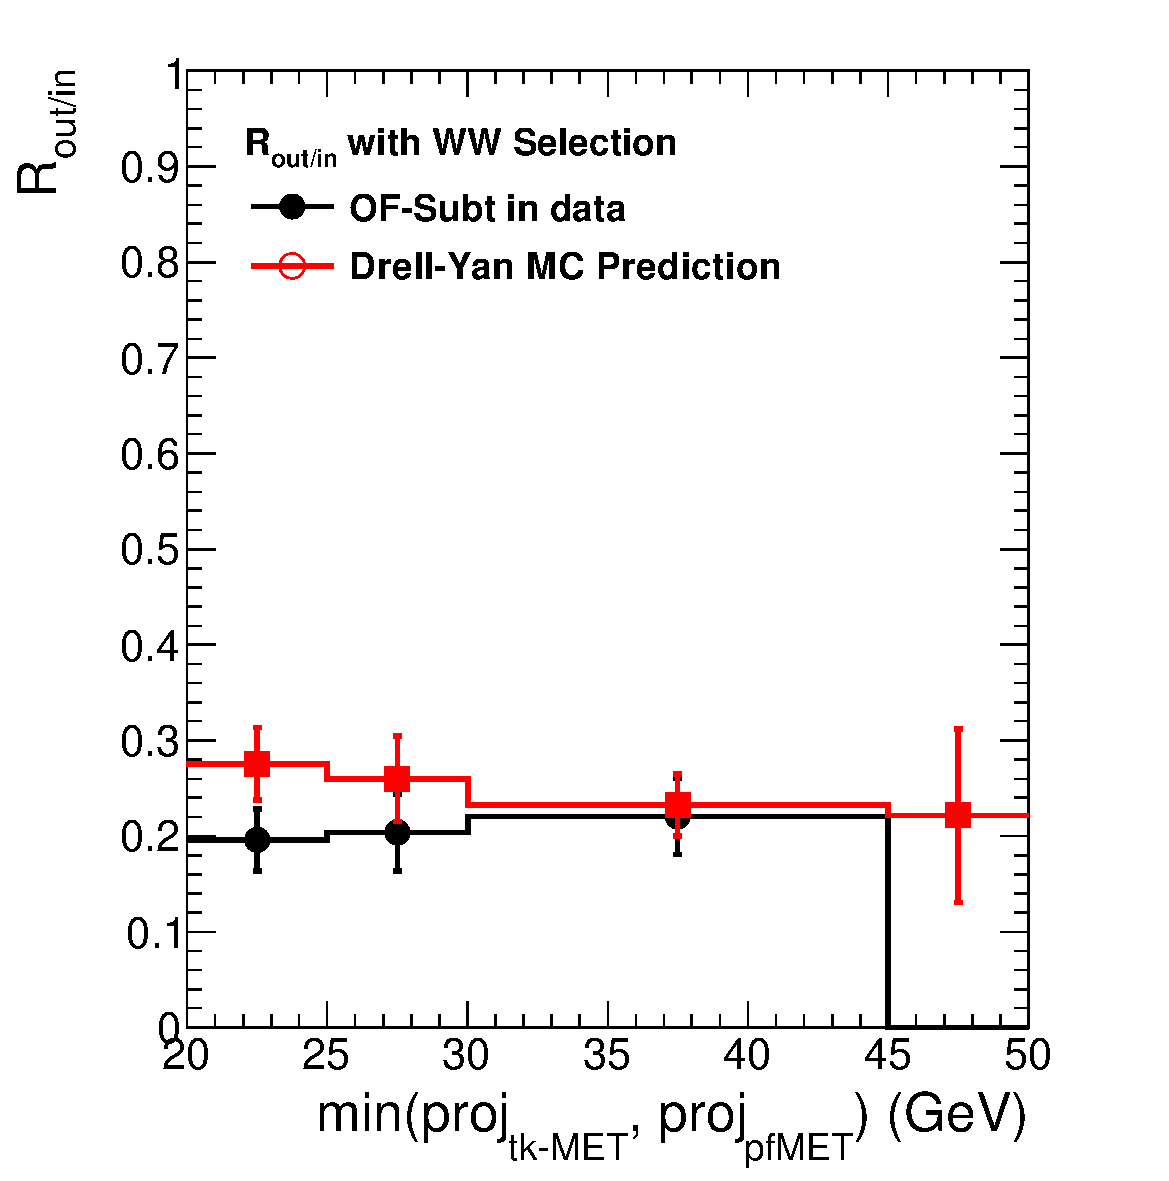
\includegraphics[width=.3\textwidth]{figures/Routin_ee_0Jet_mH0_1616pb_dy.pdf}}
\subfigure[$\mu\mu$ 0-Jet]{
\centering
\label{subfig:dyr_mm_mh0_0j}
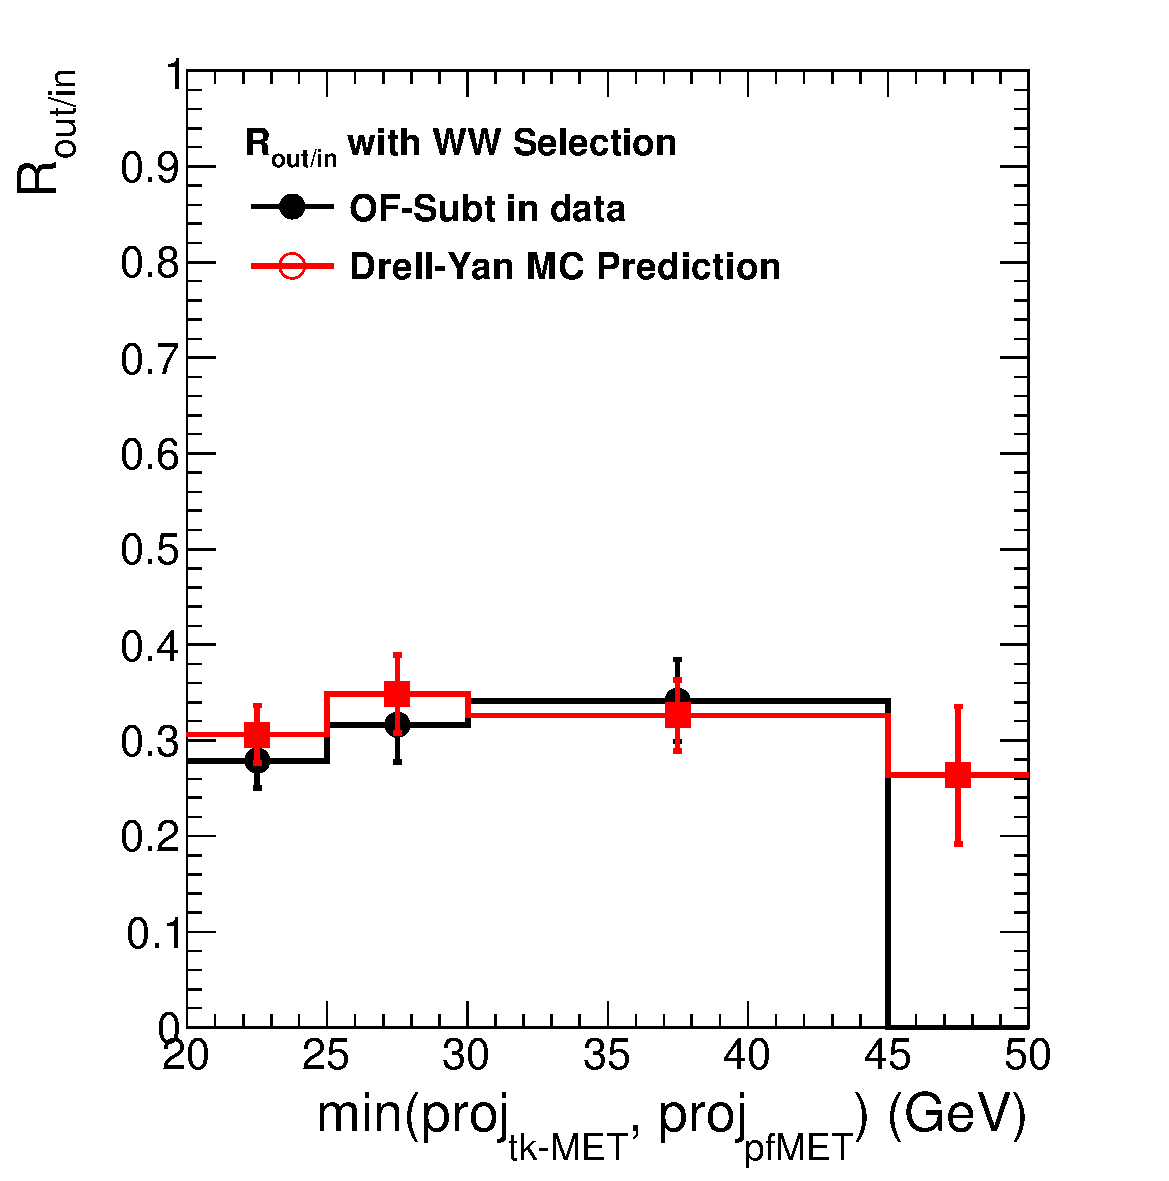
\includegraphics[width=.3\textwidth]{figures/Routin_mm_0Jet_mH0_1616pb_dy.pdf}}
\subfigure[ee and $\mu\mu$ 0-Jet]{
\centering
\label{subfig:dyr_mh0_0j}
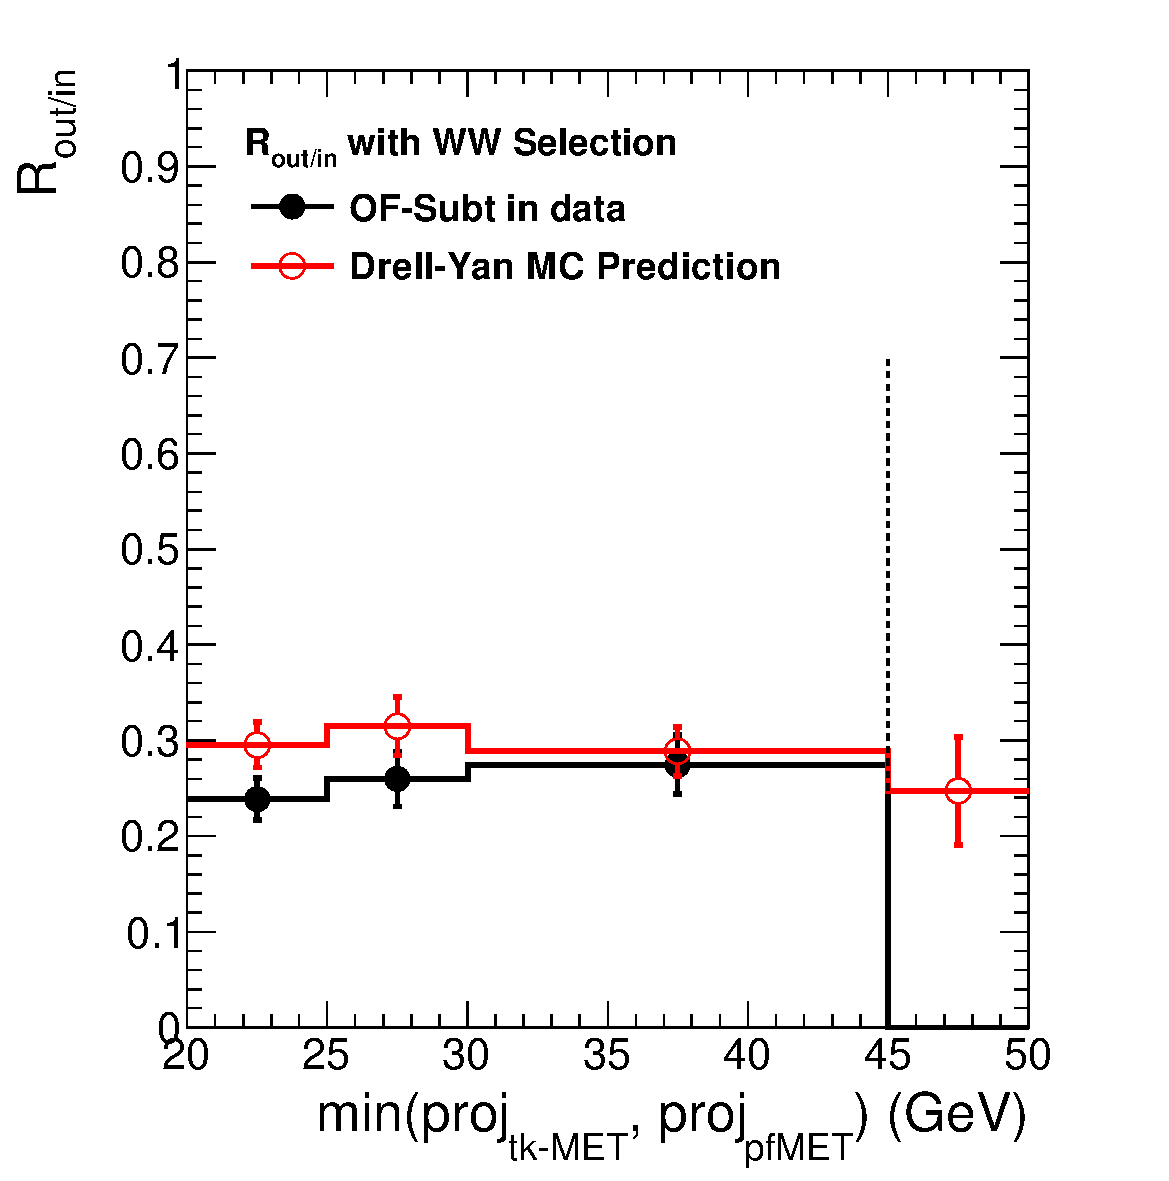
\includegraphics[width=.3\textwidth]{figures/Routin_0Jet_mH0_1616pb_dy.pdf}}
\centering
\subfigure[ee 1-Jet]{
\centering
\label{subfig:dyr_ee_mh0_1j}
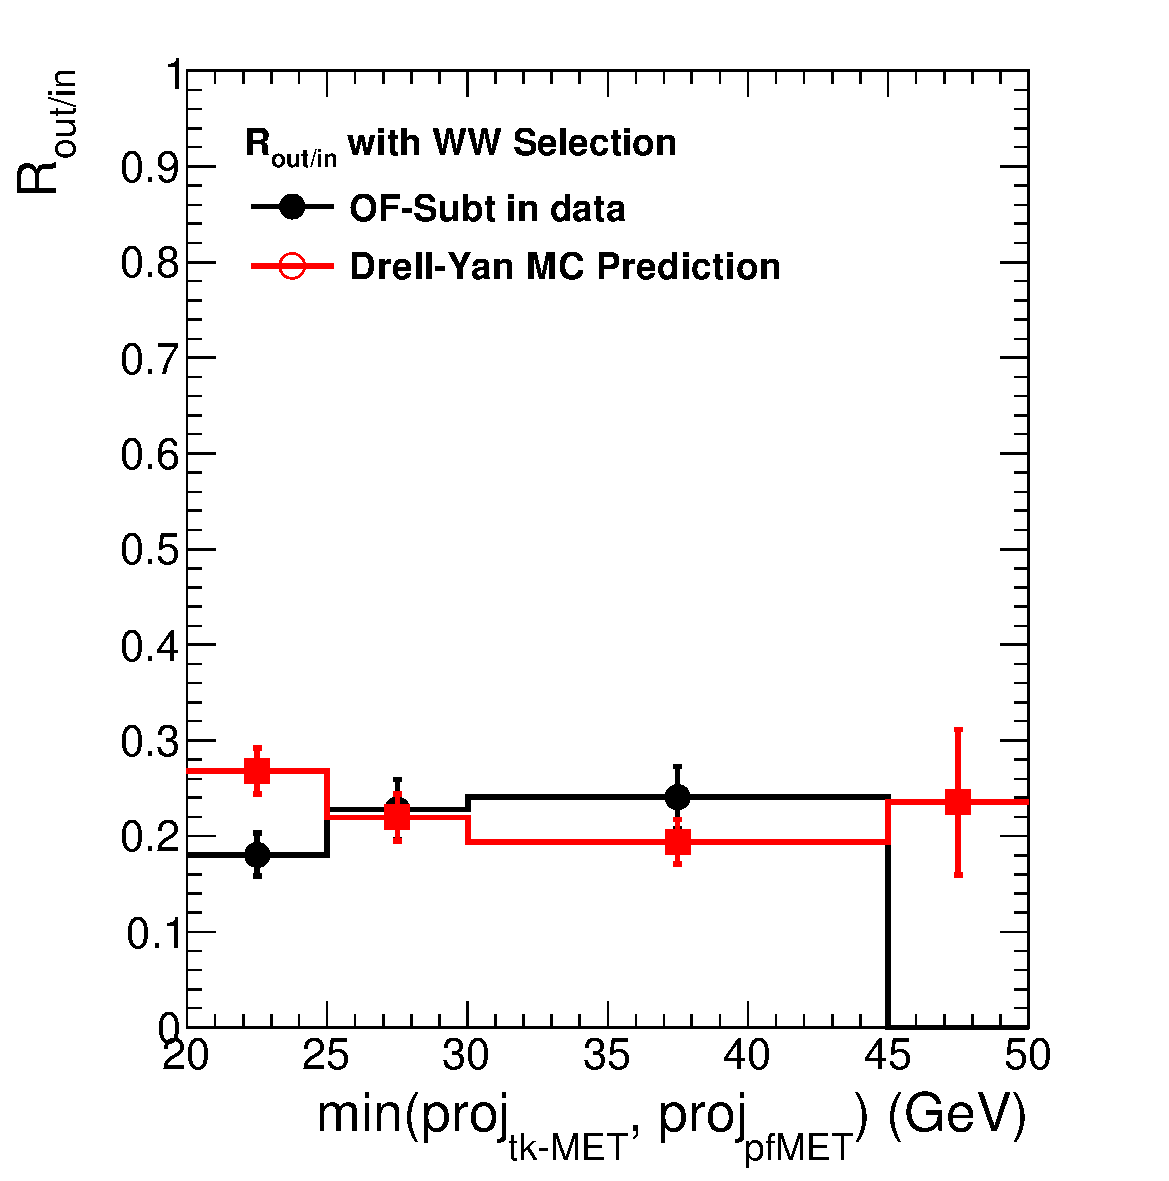
\includegraphics[width=.3\textwidth]{figures/Routin_ee_1Jet_mH0_1616pb_dy.pdf}}
\subfigure[$\mu\mu$ 1-Jet]{
\centering
\label{subfig:dyr_mm_mh0_1j}
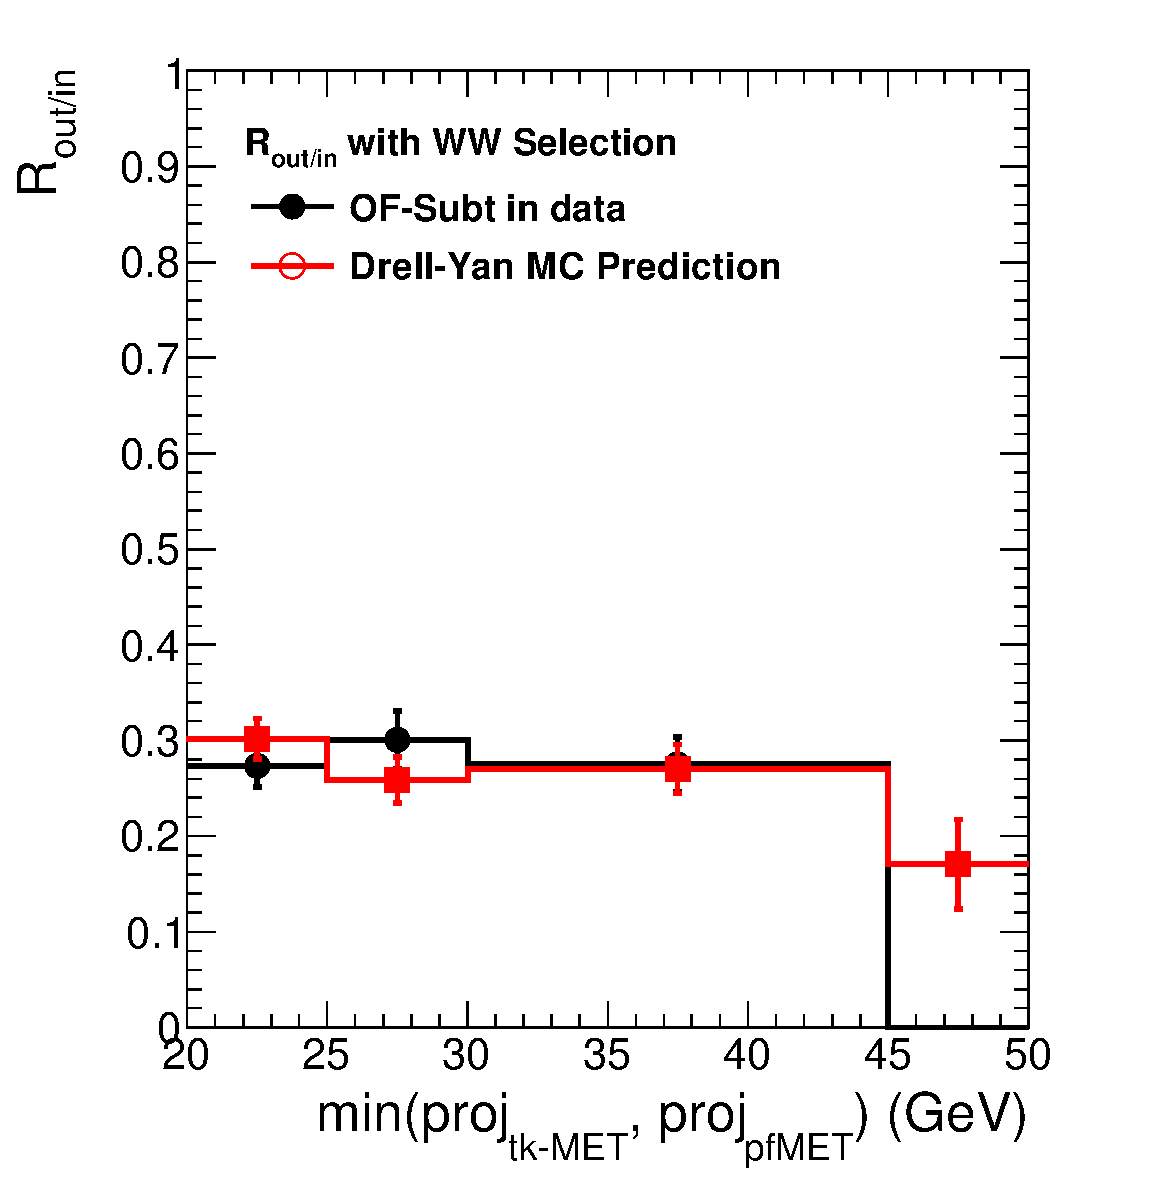
\includegraphics[width=.3\textwidth]{figures/Routin_mm_1Jet_mH0_1616pb_dy.pdf}}
\subfigure[ee and$\mu\mu$ 1-Jet]{
\centering
\label{subfig:dyr_mh0_1j}
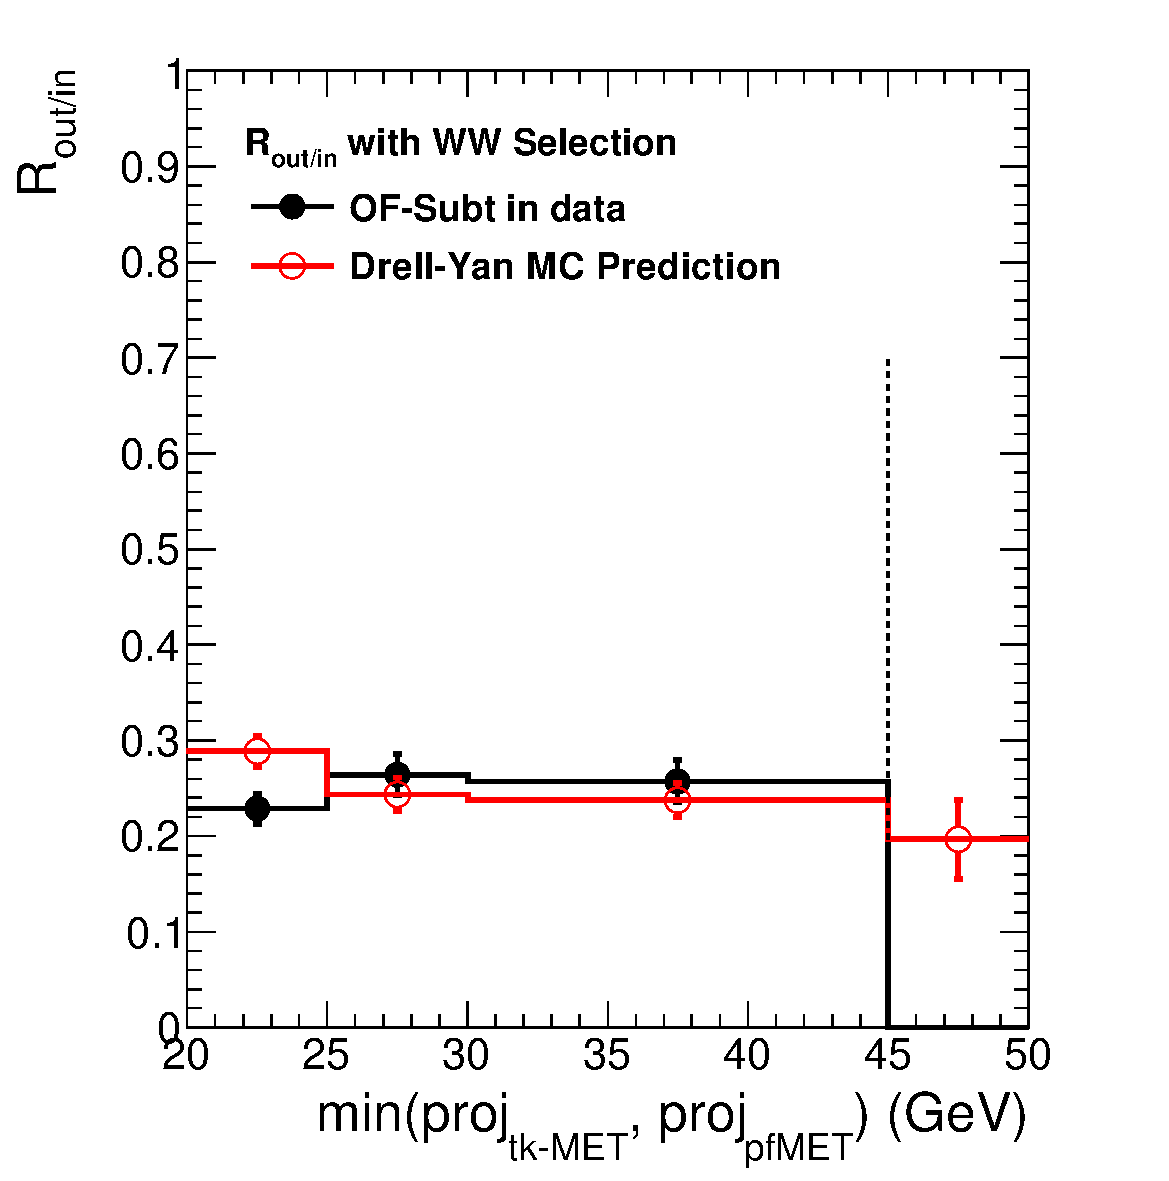
\includegraphics[width=.3\textwidth]{figures/Routin_1Jet_mH0_1616pb_dy.pdf}}
\subfigure[ee 2-Jet]{
\centering
\label{subfig:dyr_ee_mh0_2j}
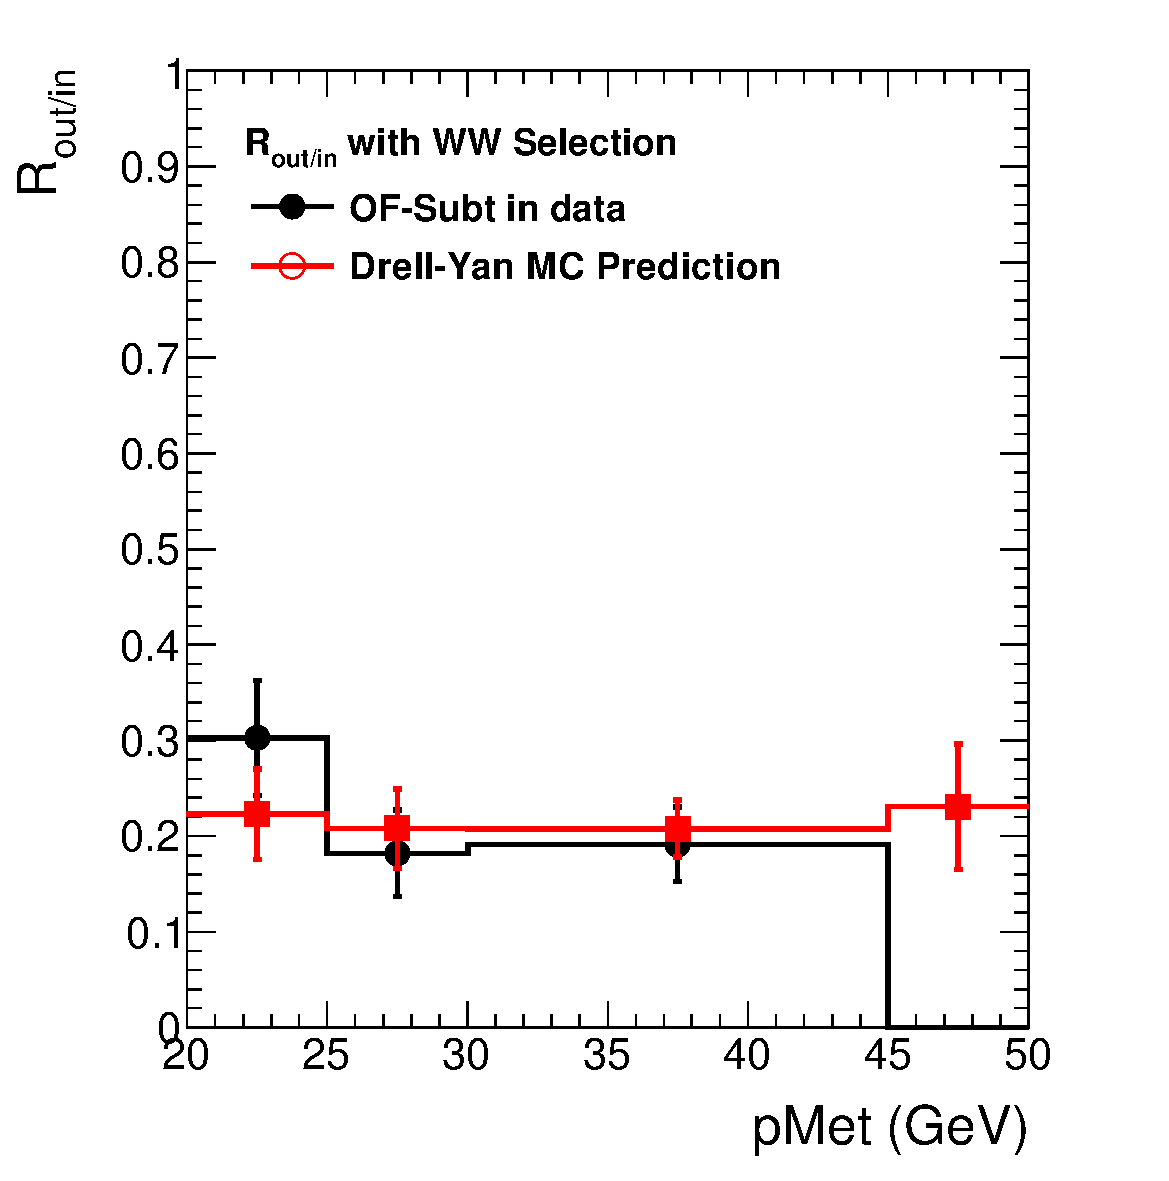
\includegraphics[width=.3\textwidth]{figures/Routin_ee_2Jet_mH0_1616pb_dy.pdf}}
\subfigure[$\mu\mu$ 2-Jet]{
\centering
\label{subfig:dyr_mm_mh0_2j}
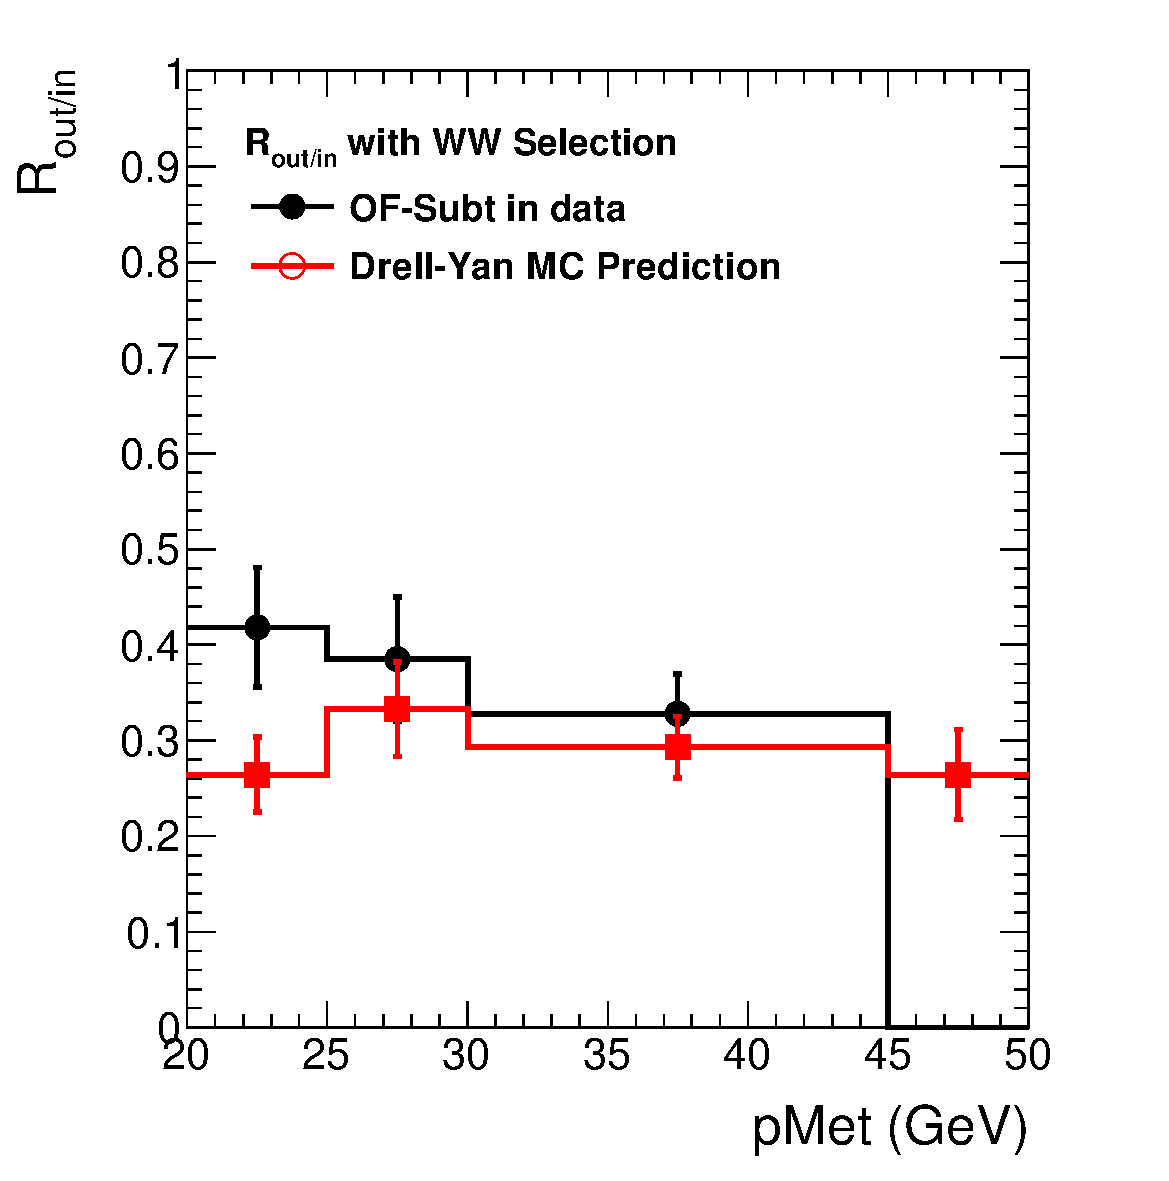
\includegraphics[width=.3\textwidth]{figures/Routin_mm_2Jet_mH0_1616pb_dy.pdf}}
\subfigure[ee and $\mu\mu$ 2-Jet]{
\centering
\label{subfig:dyr_mh0_2j}
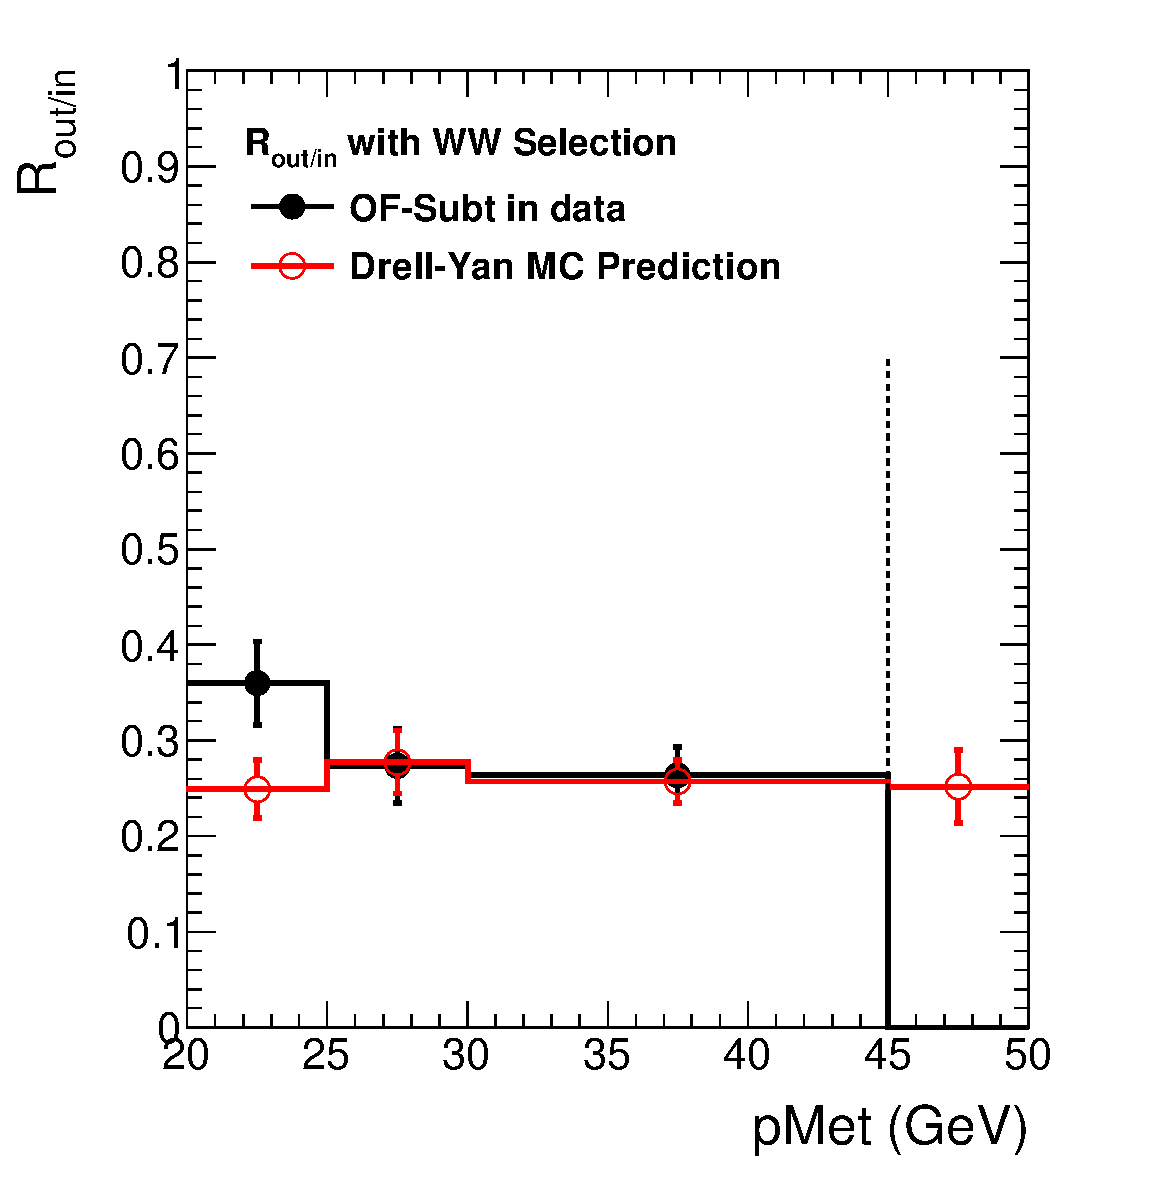
\includegraphics[width=.3\textwidth]{figures/Routin_2Jet_mH0_1616pb_dy.pdf}}
\caption{
 The \routin\, as a function of MET measured from data (black solid dots) 
and MC (red open circles) for the Drell-Yan processes after the WW preselections. 
The measurements in data are done using the opposite flavor subtraction method. }
\label{fig:dyr_hww}
\end{figure}

\begin{figure}[!htbp]
\begin{center}$
\begin{array}{cccc}
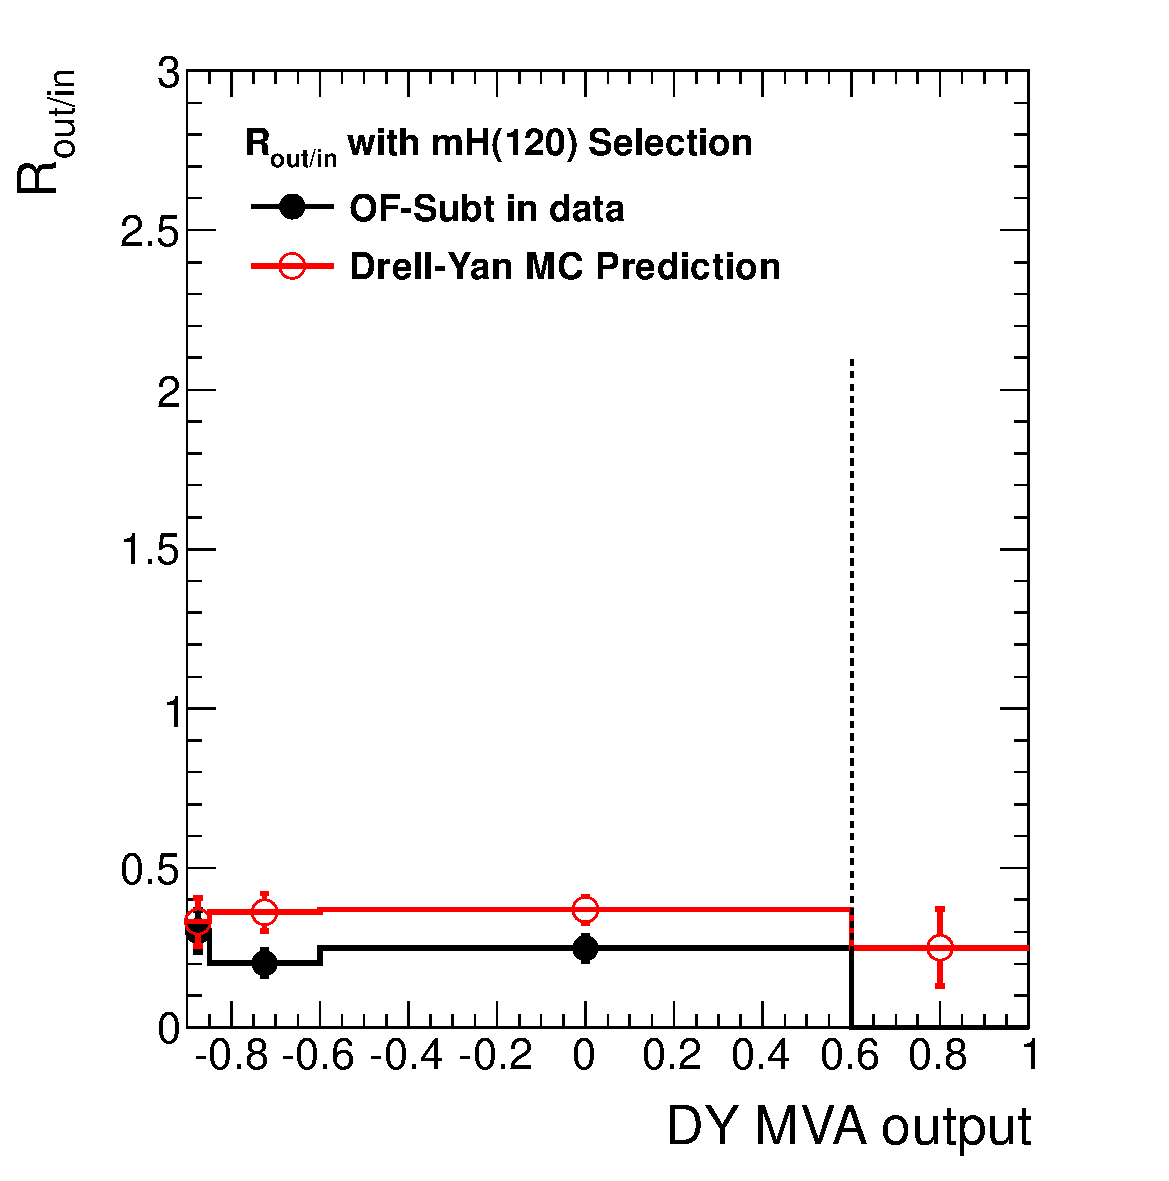
\includegraphics[width=.29\textwidth]{figures/Routin_0Jet_mH120_1616pb_dy.pdf} & 
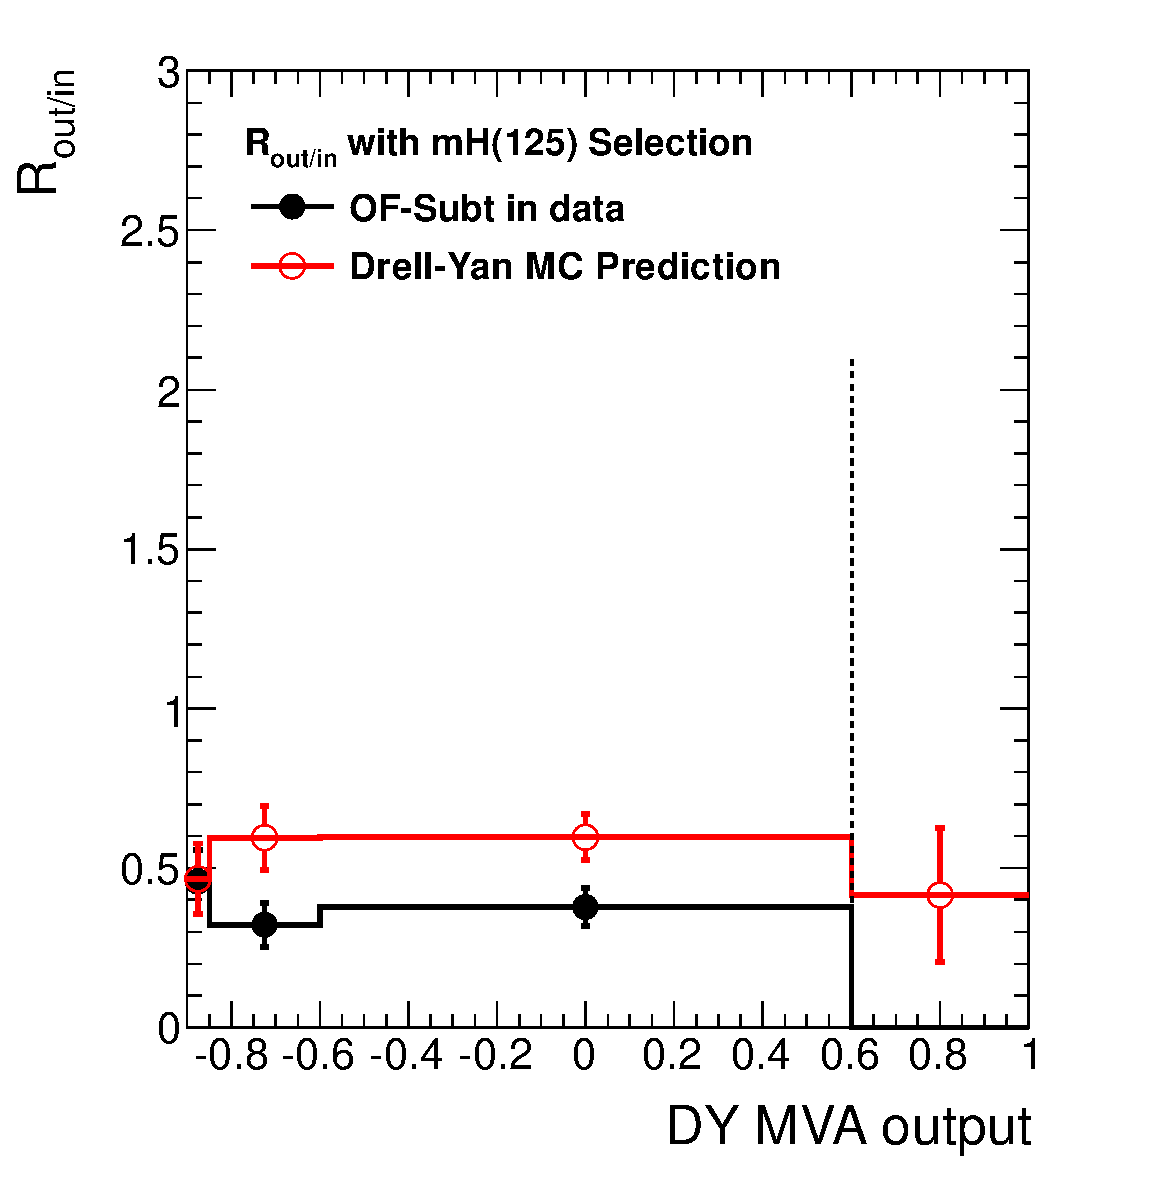
\includegraphics[width=.29\textwidth]{figures/Routin_0Jet_mH125_1616pb_dy.pdf} & 
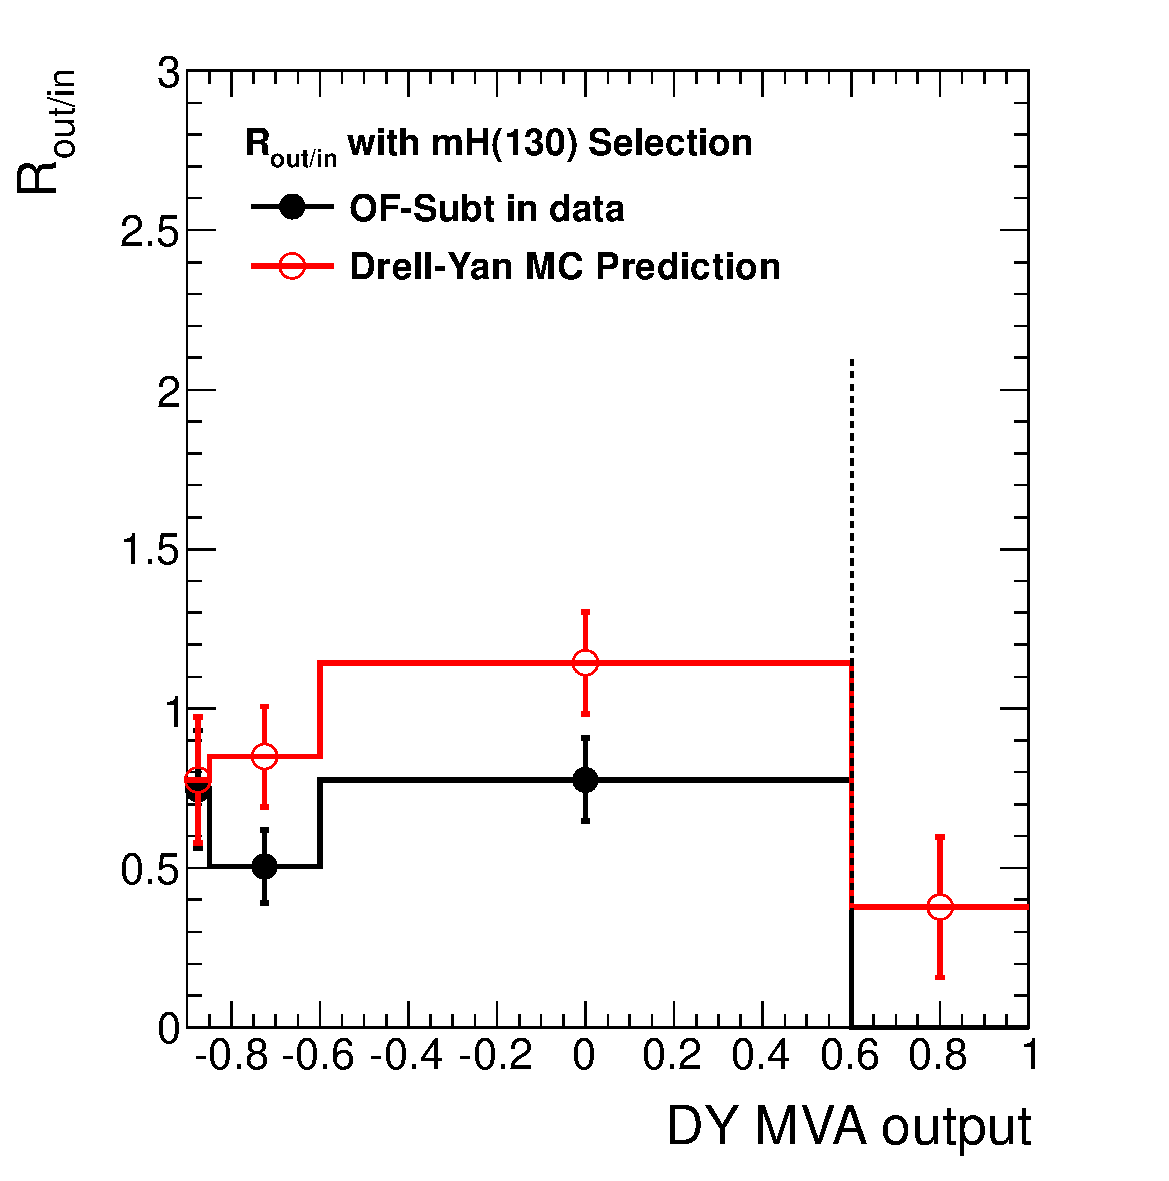
\includegraphics[width=.29\textwidth]{figures/Routin_0Jet_mH130_1616pb_dy.pdf} \\
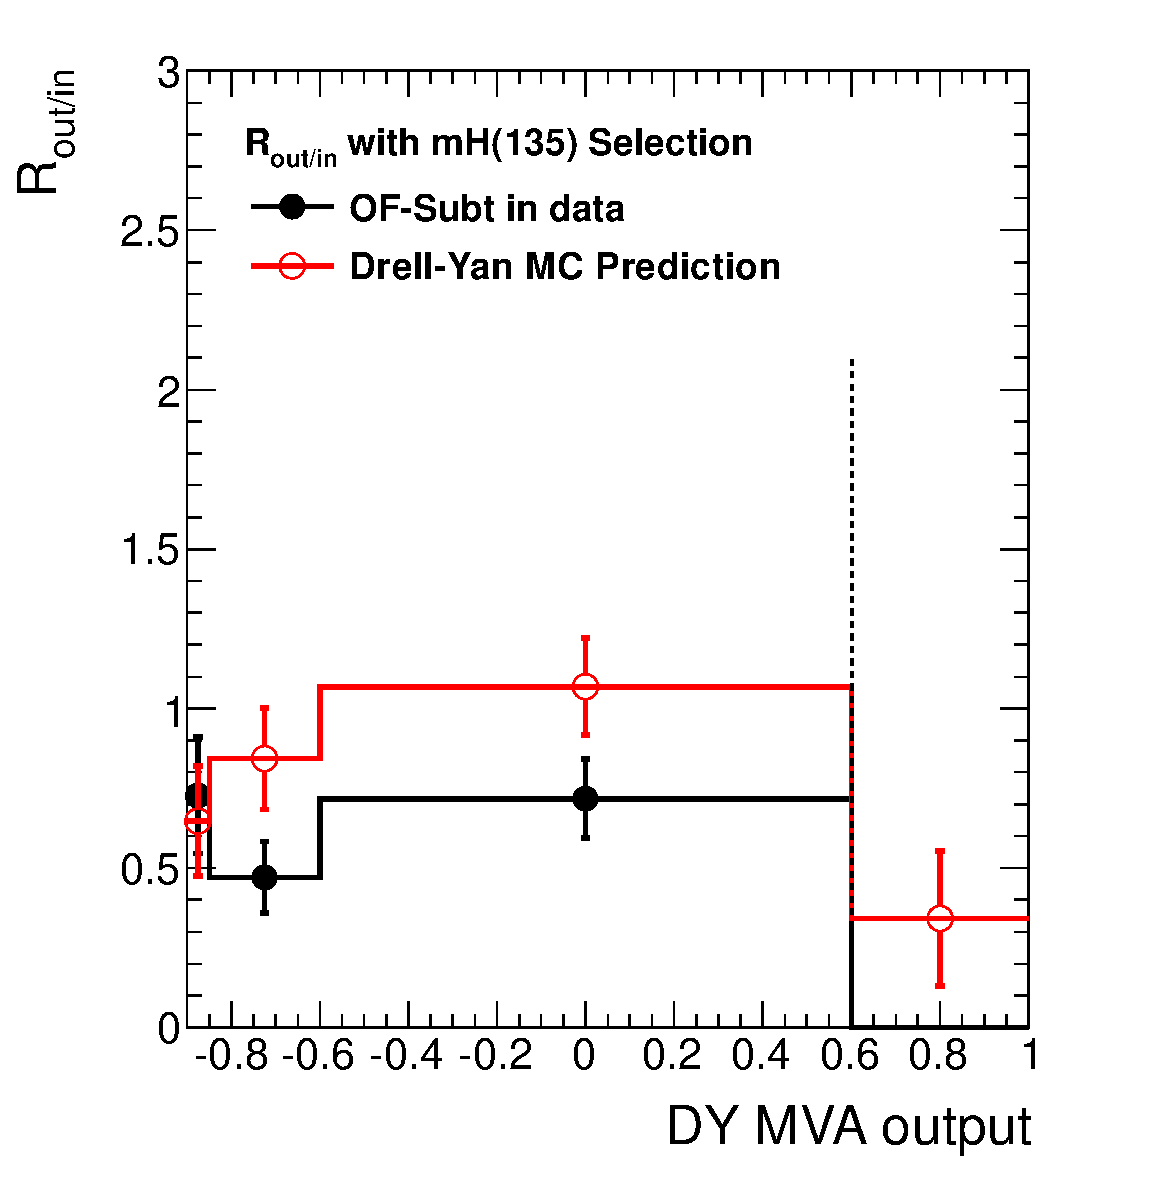
\includegraphics[width=.29\textwidth]{figures/Routin_0Jet_mH135_1616pb_dy.pdf} & 
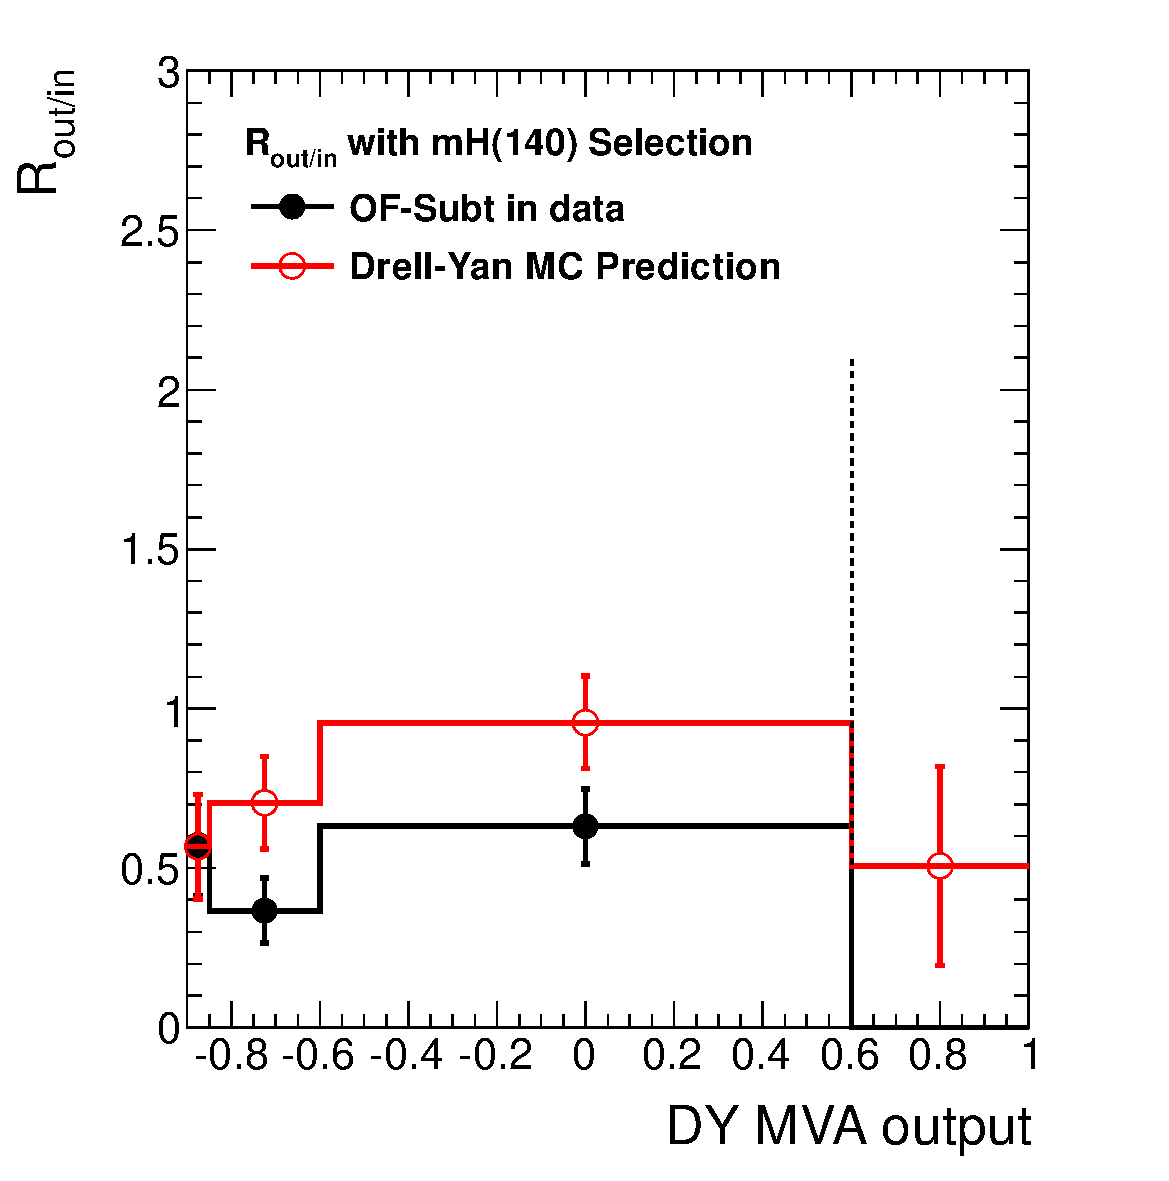
\includegraphics[width=.29\textwidth]{figures/Routin_0Jet_mH140_1616pb_dy.pdf} & 
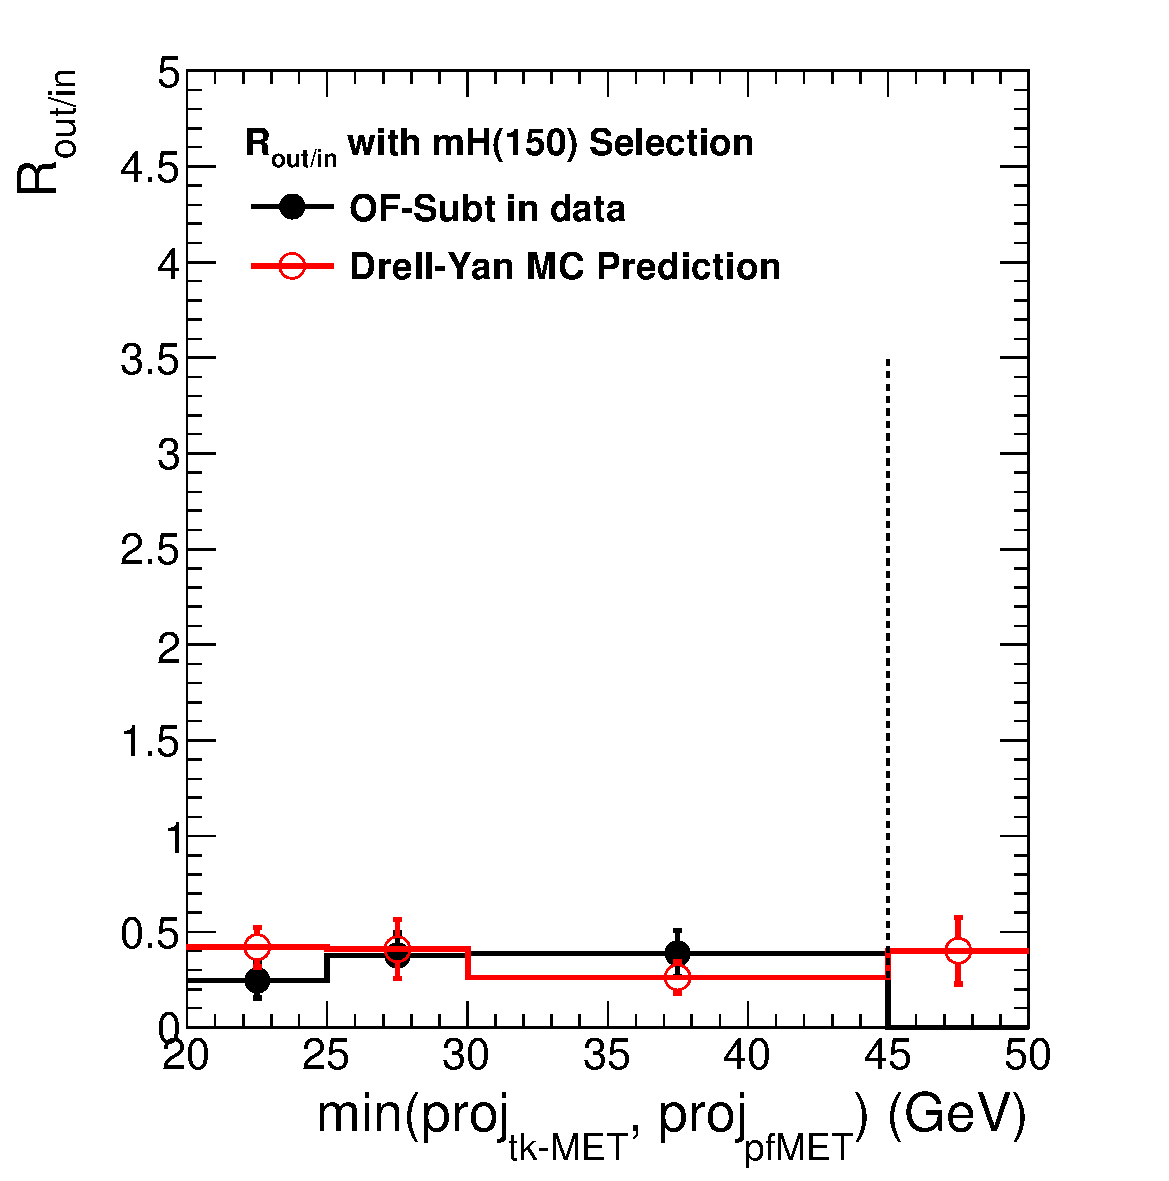
\includegraphics[width=.29\textwidth]{figures/Routin_0Jet_mH150_1616pb_dy.pdf} \\
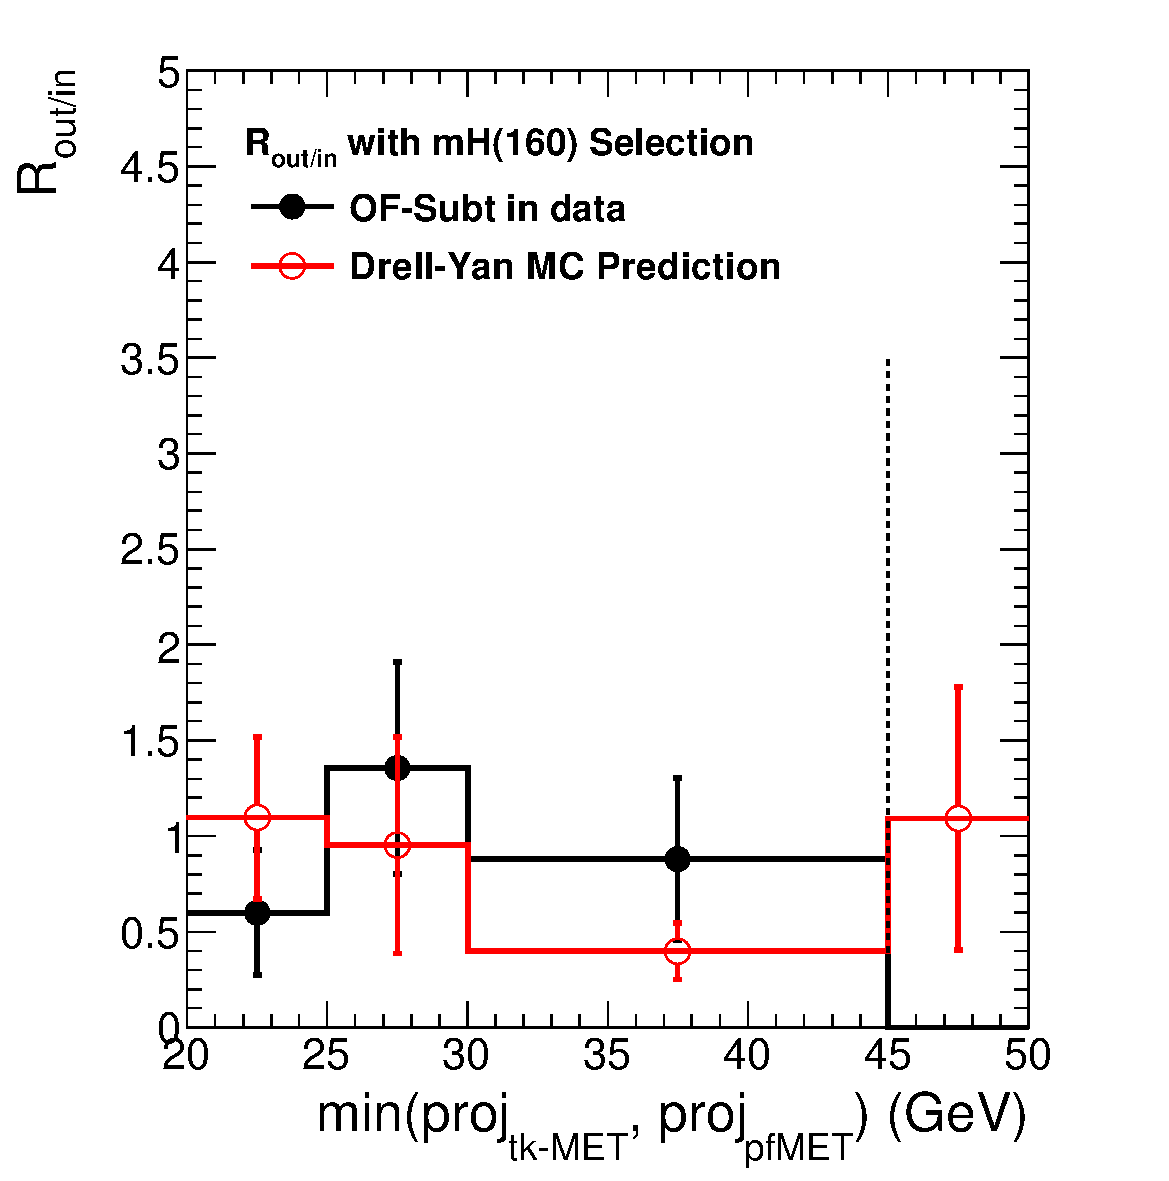
\includegraphics[width=.29\textwidth]{figures/Routin_0Jet_mH160_1616pb_dy.pdf} &
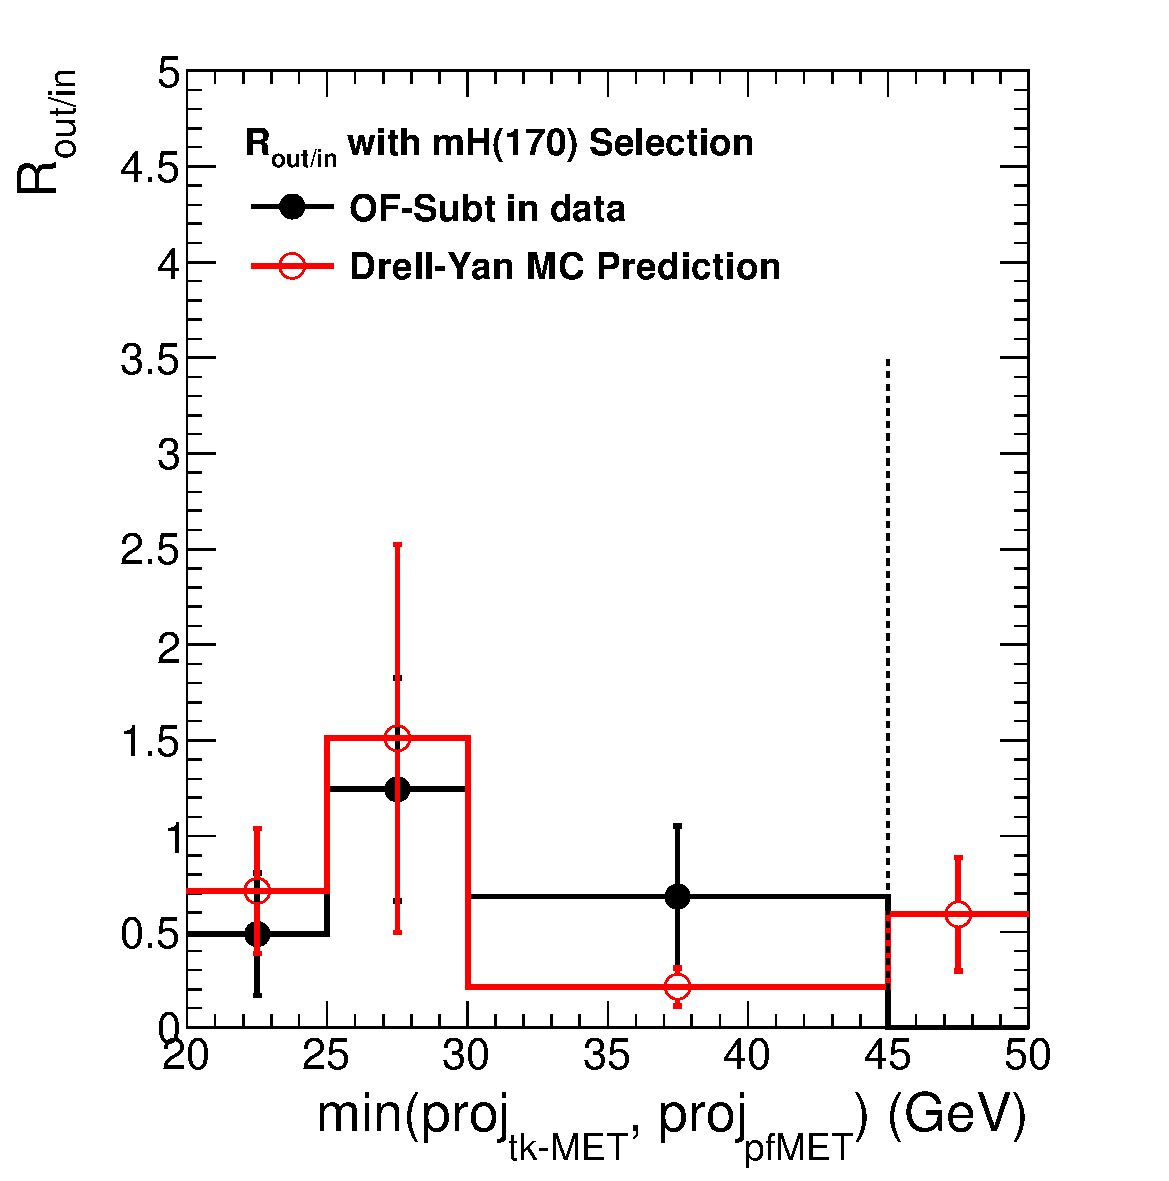
\includegraphics[width=.29\textwidth]{figures/Routin_0Jet_mH170_1616pb_dy.pdf} &
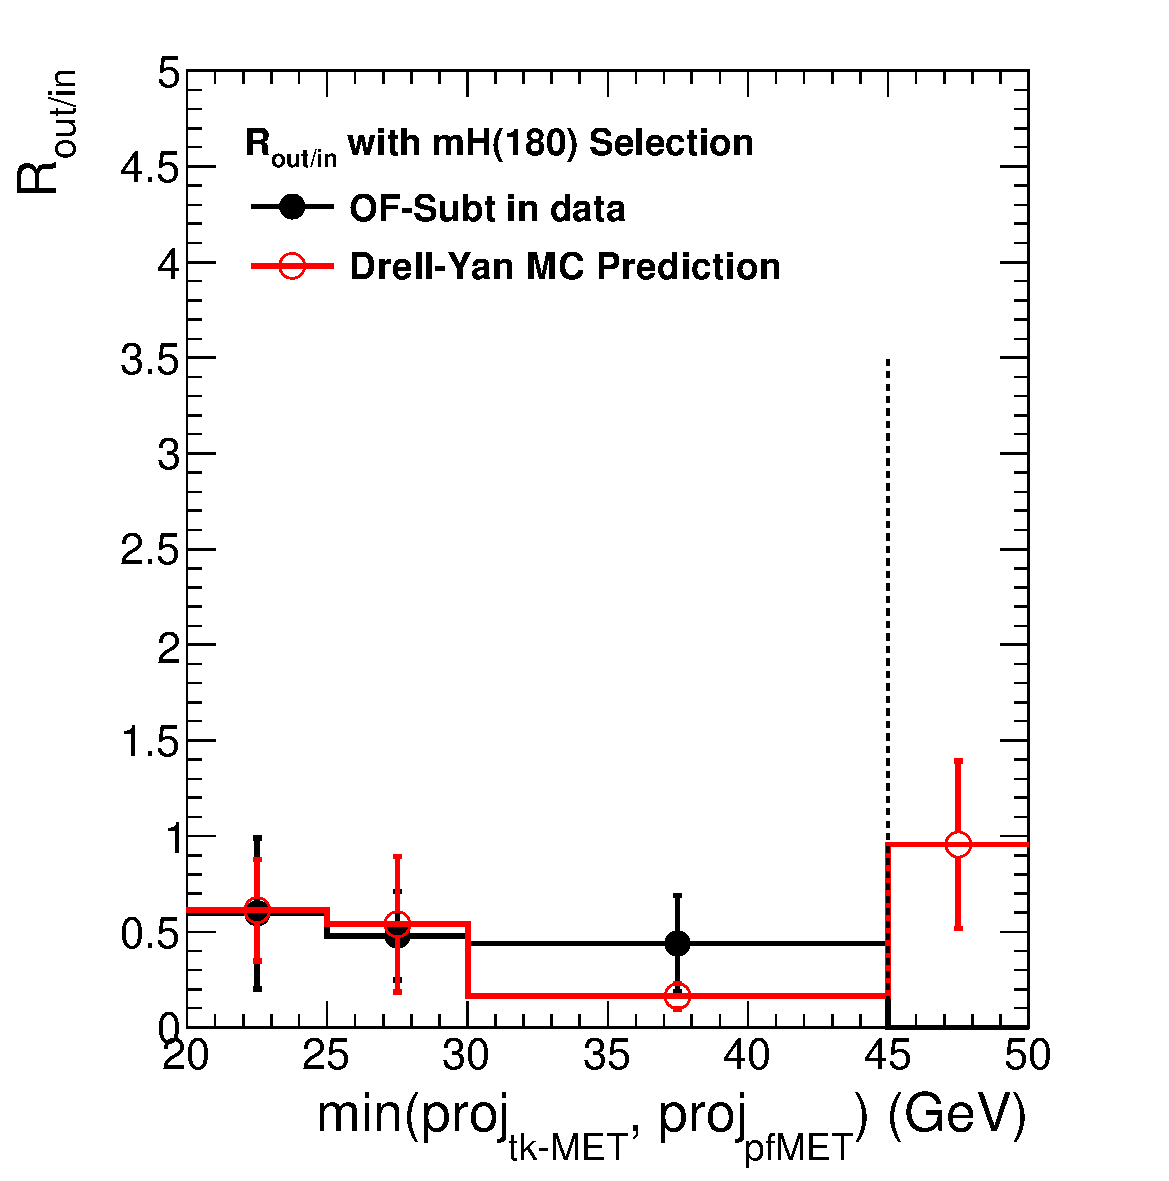
\includegraphics[width=.29\textwidth]{figures/Routin_0Jet_mH180_1616pb_dy.pdf} \\
\end{array}$
\caption{ The \routin\, (ee and $\mu\mu$ combined) as a function of MET measured from data (black solid dots) 
and MC (red open circles) for the Drell-Yan processes in the 0-Jet bin at the 
Higgs selection level in the cut-based analysis. 
The measurements in data are performed using the opposite flavor subtraction method. 
The difference in the \routin measurements in different higg selections are due to the 
different kinematic cuts applied. 
}
\label{fig:routin_0jet}
\end{center}
\end{figure}


\begin{figure}[!htbp]
\begin{center}$
\begin{array}{cccc}
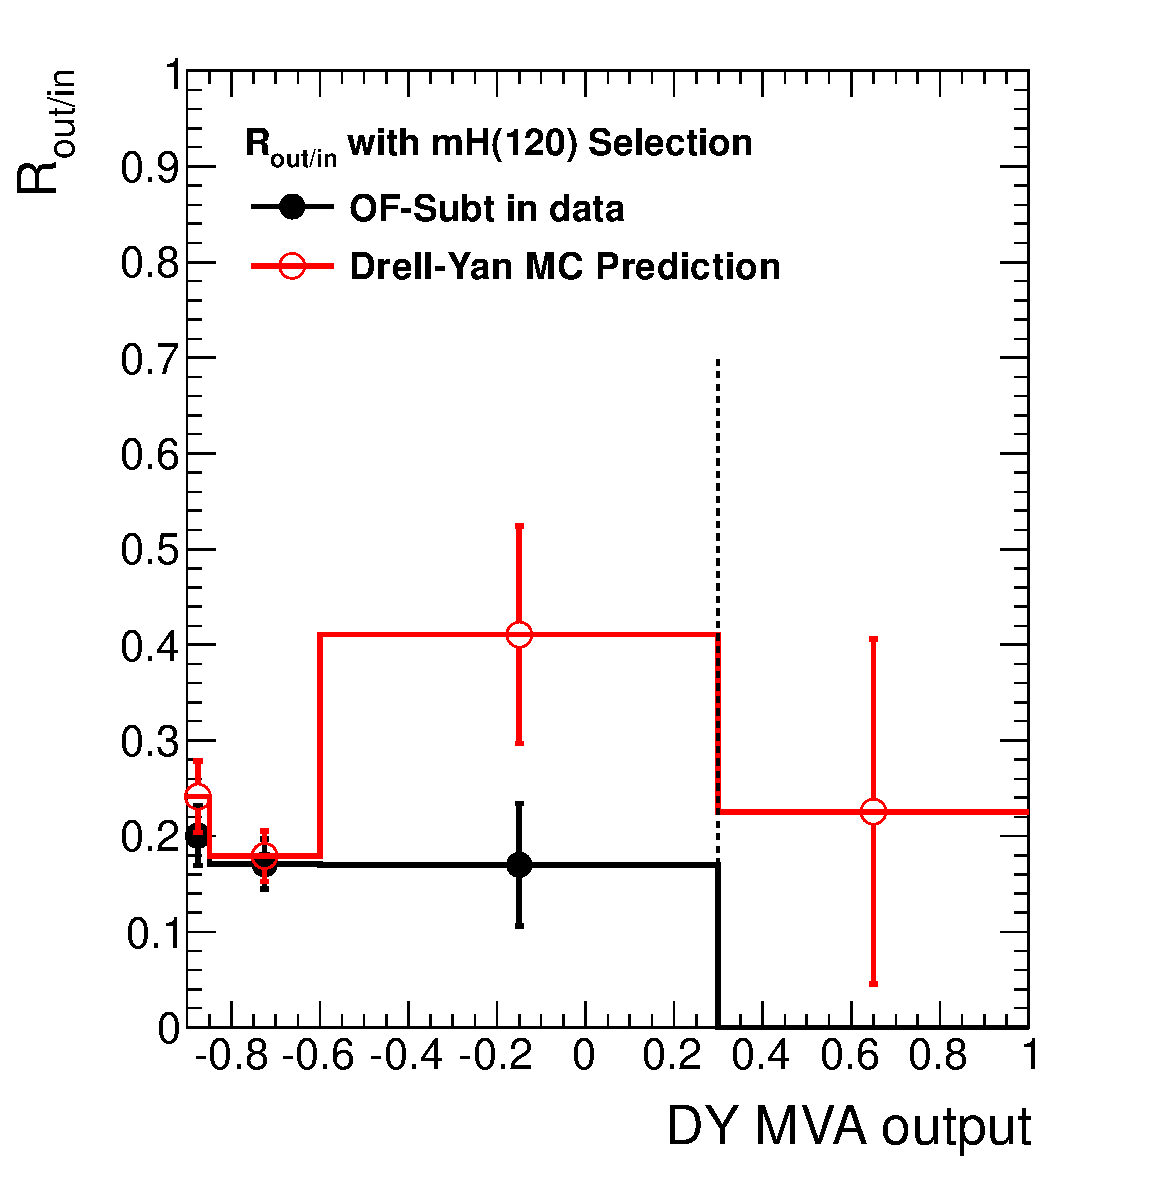
\includegraphics[width=.29\textwidth]{figures/Routin_1Jet_mH120_1616pb_dy.pdf} & 
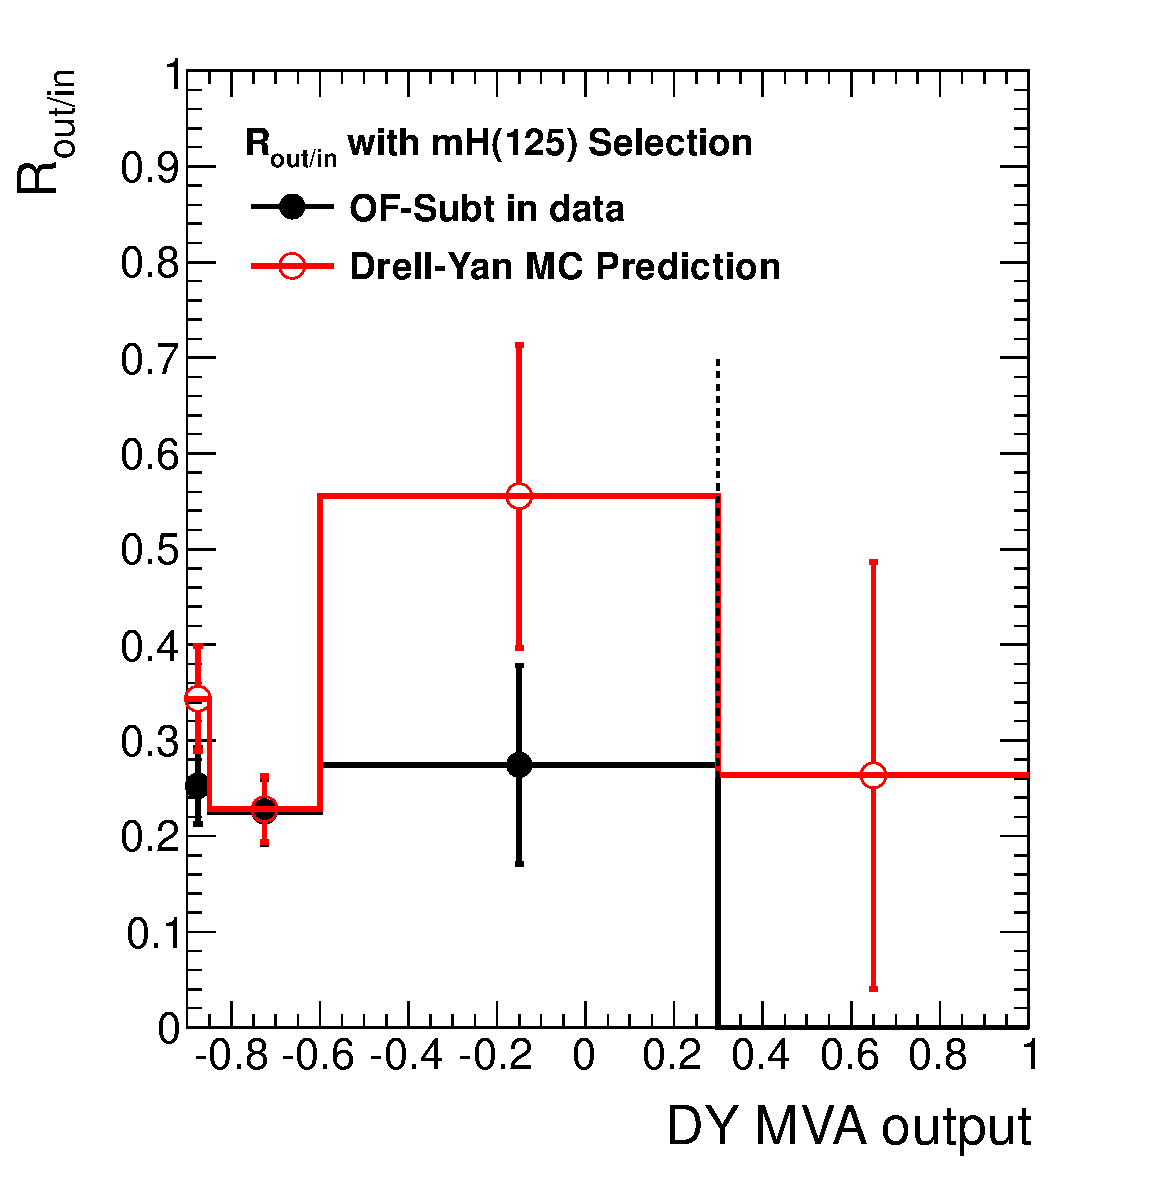
\includegraphics[width=.29\textwidth]{figures/Routin_1Jet_mH125_1616pb_dy.pdf} & 
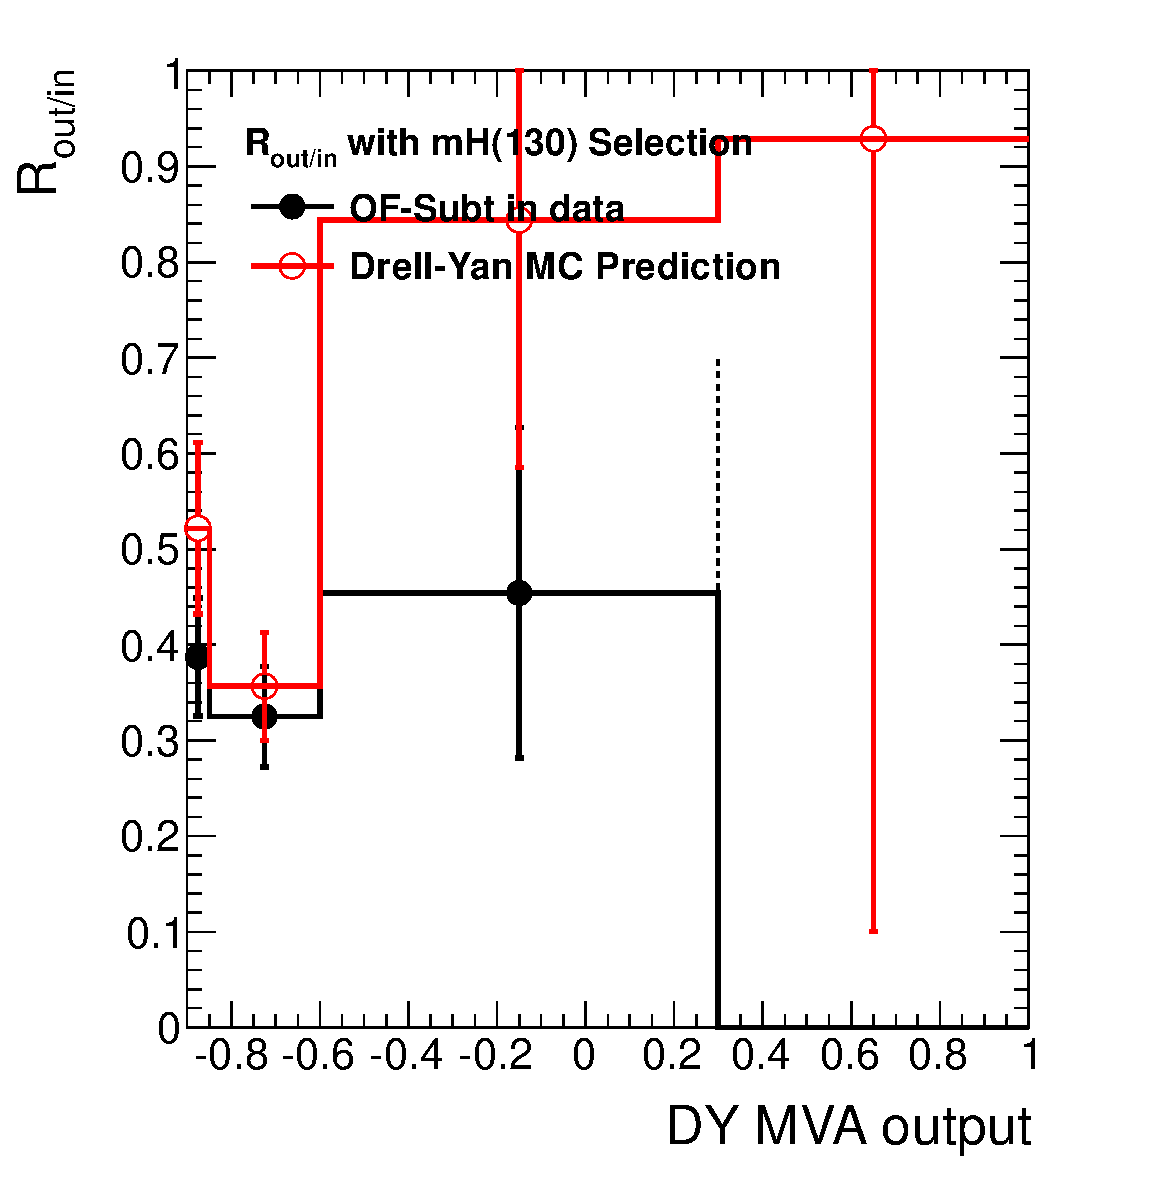
\includegraphics[width=.29\textwidth]{figures/Routin_1Jet_mH130_1616pb_dy.pdf} \\
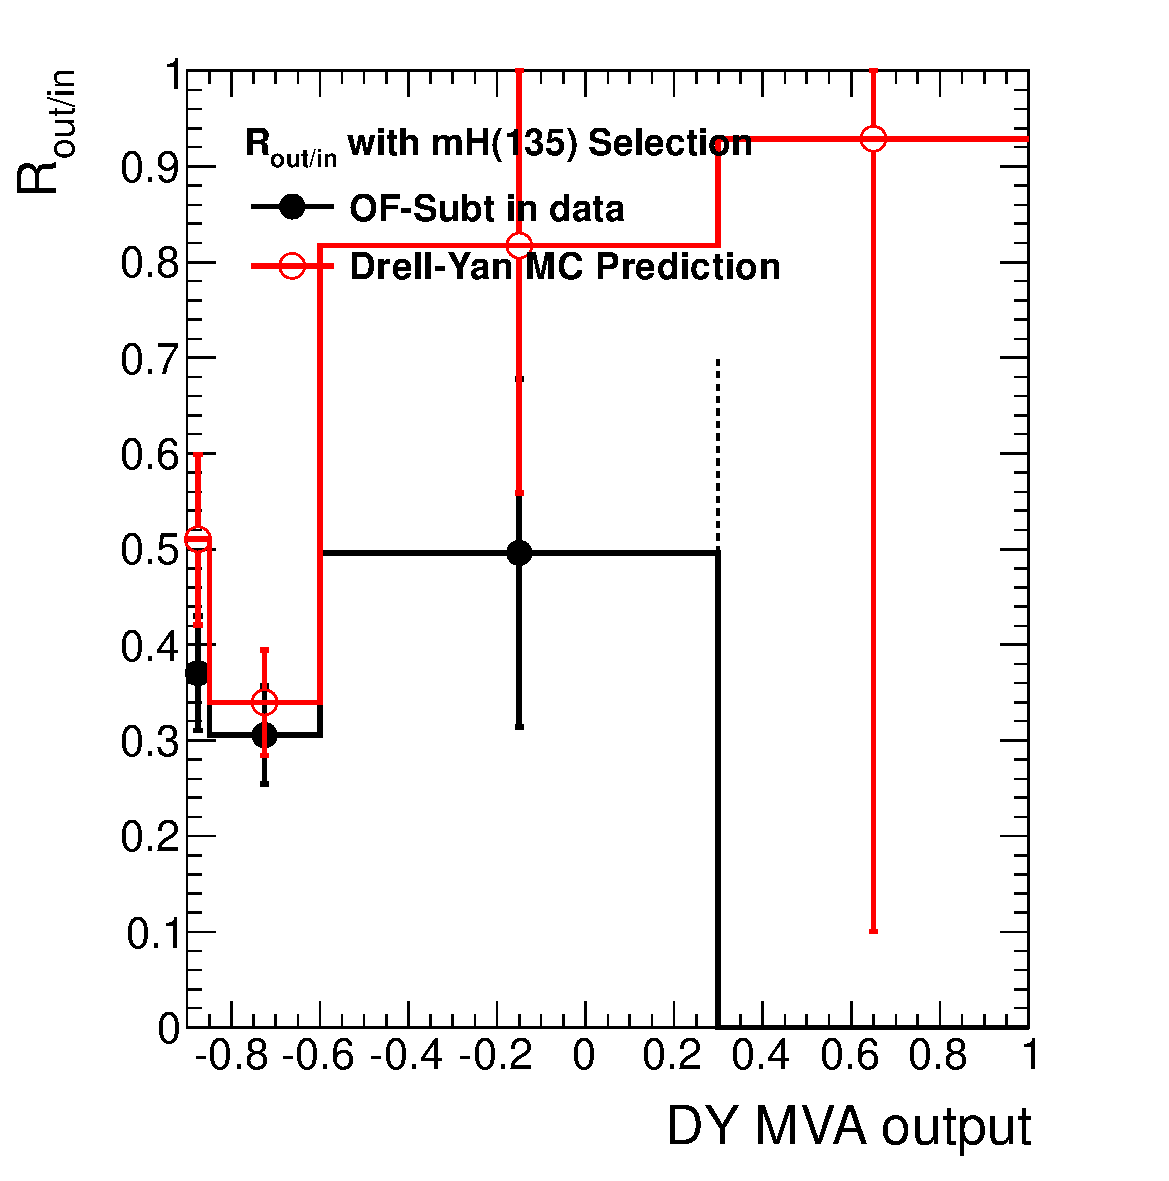
\includegraphics[width=.29\textwidth]{figures/Routin_1Jet_mH135_1616pb_dy.pdf} & 
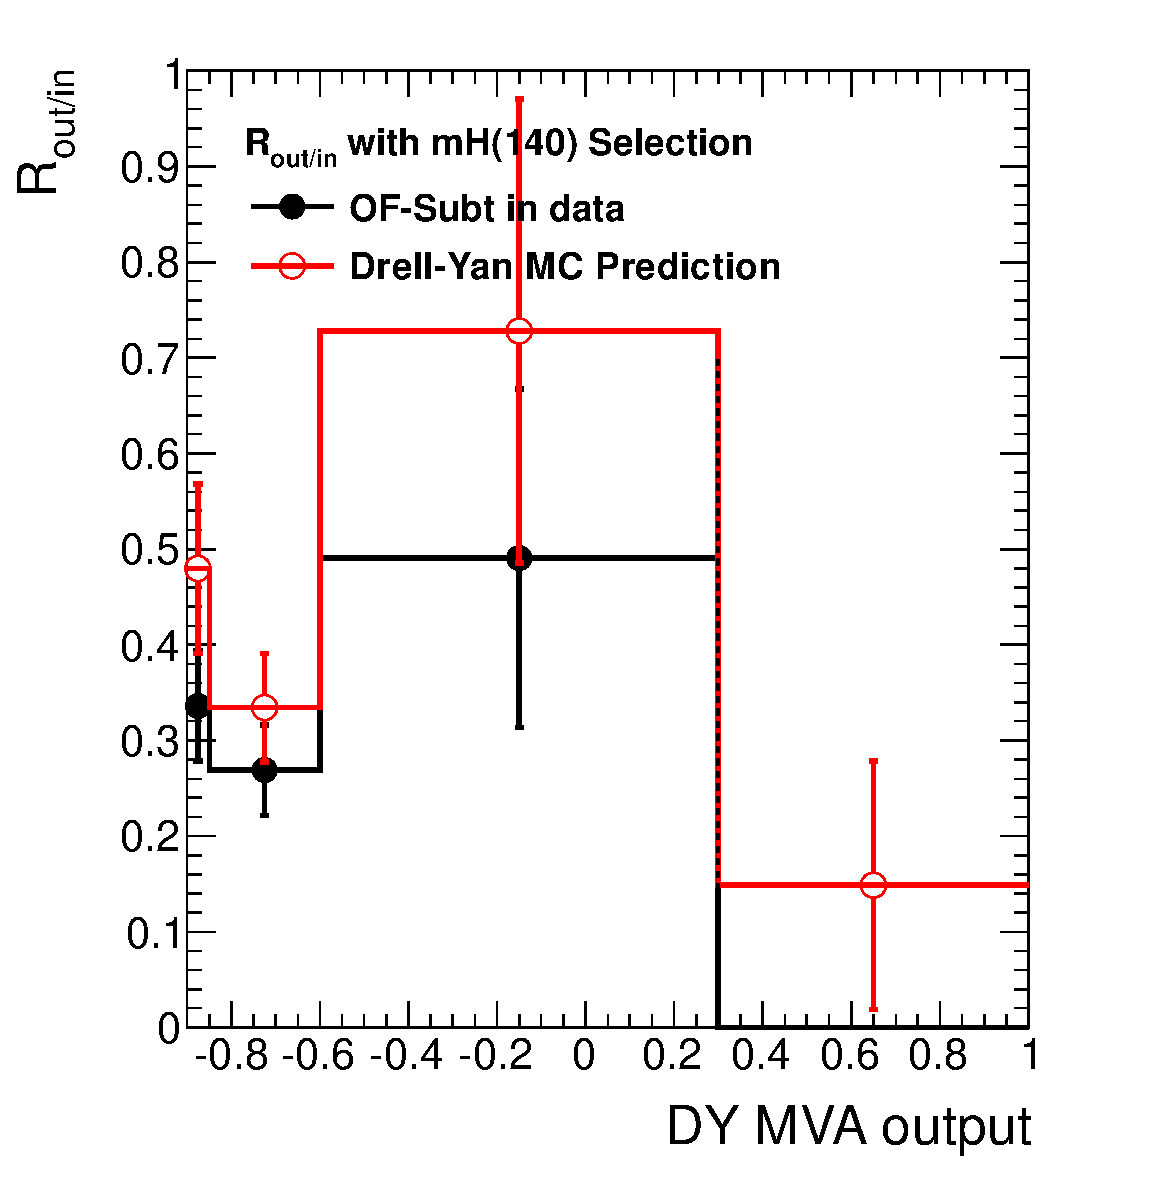
\includegraphics[width=.29\textwidth]{figures/Routin_1Jet_mH140_1616pb_dy.pdf} & 
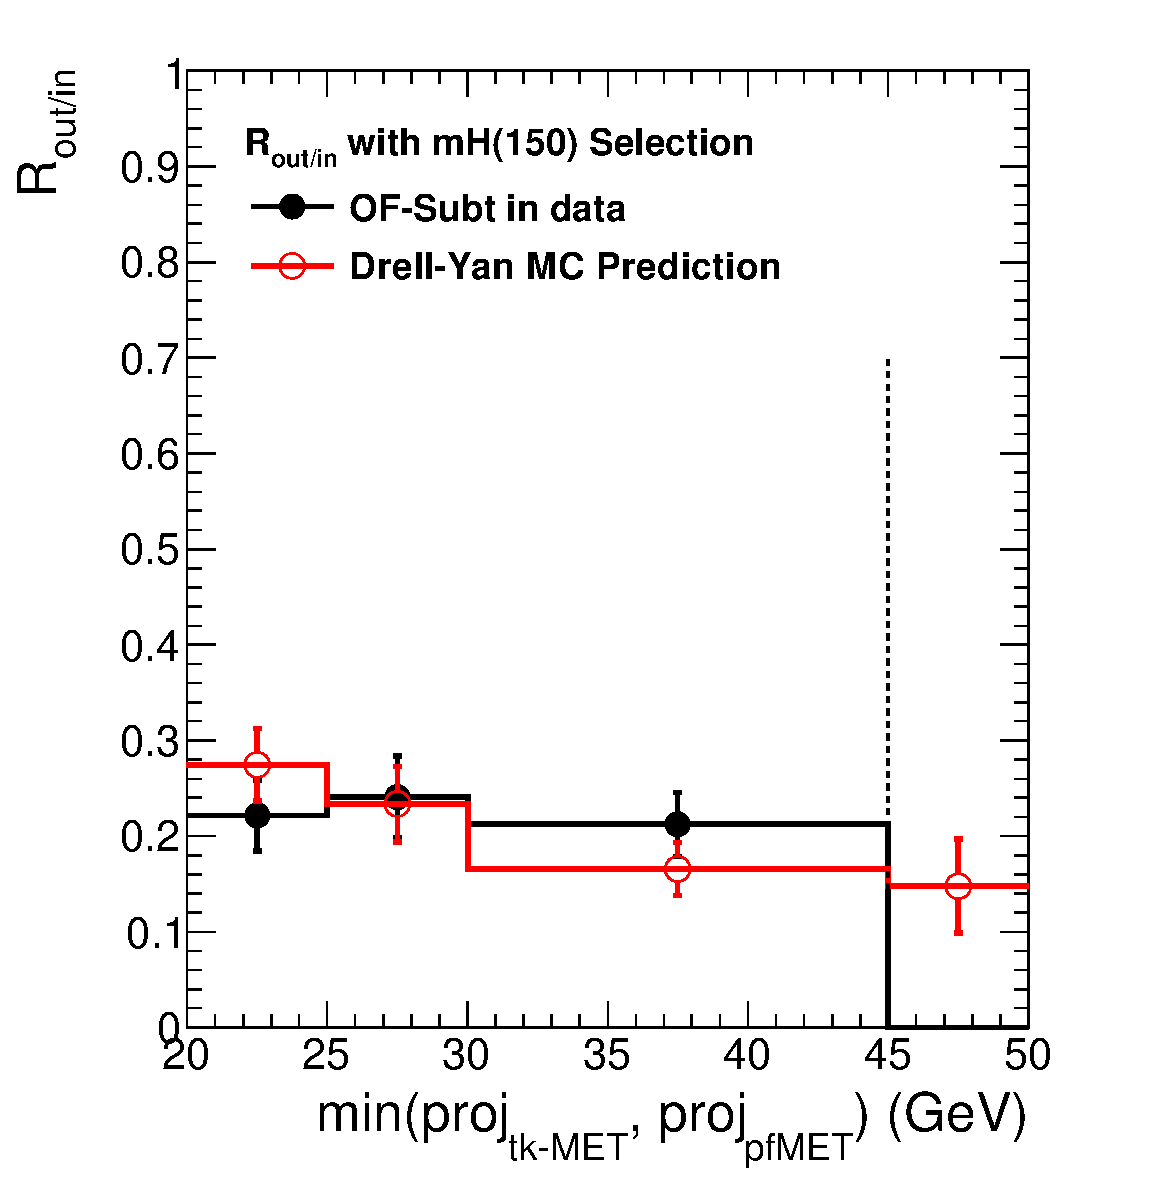
\includegraphics[width=.29\textwidth]{figures/Routin_1Jet_mH150_1616pb_dy.pdf} \\
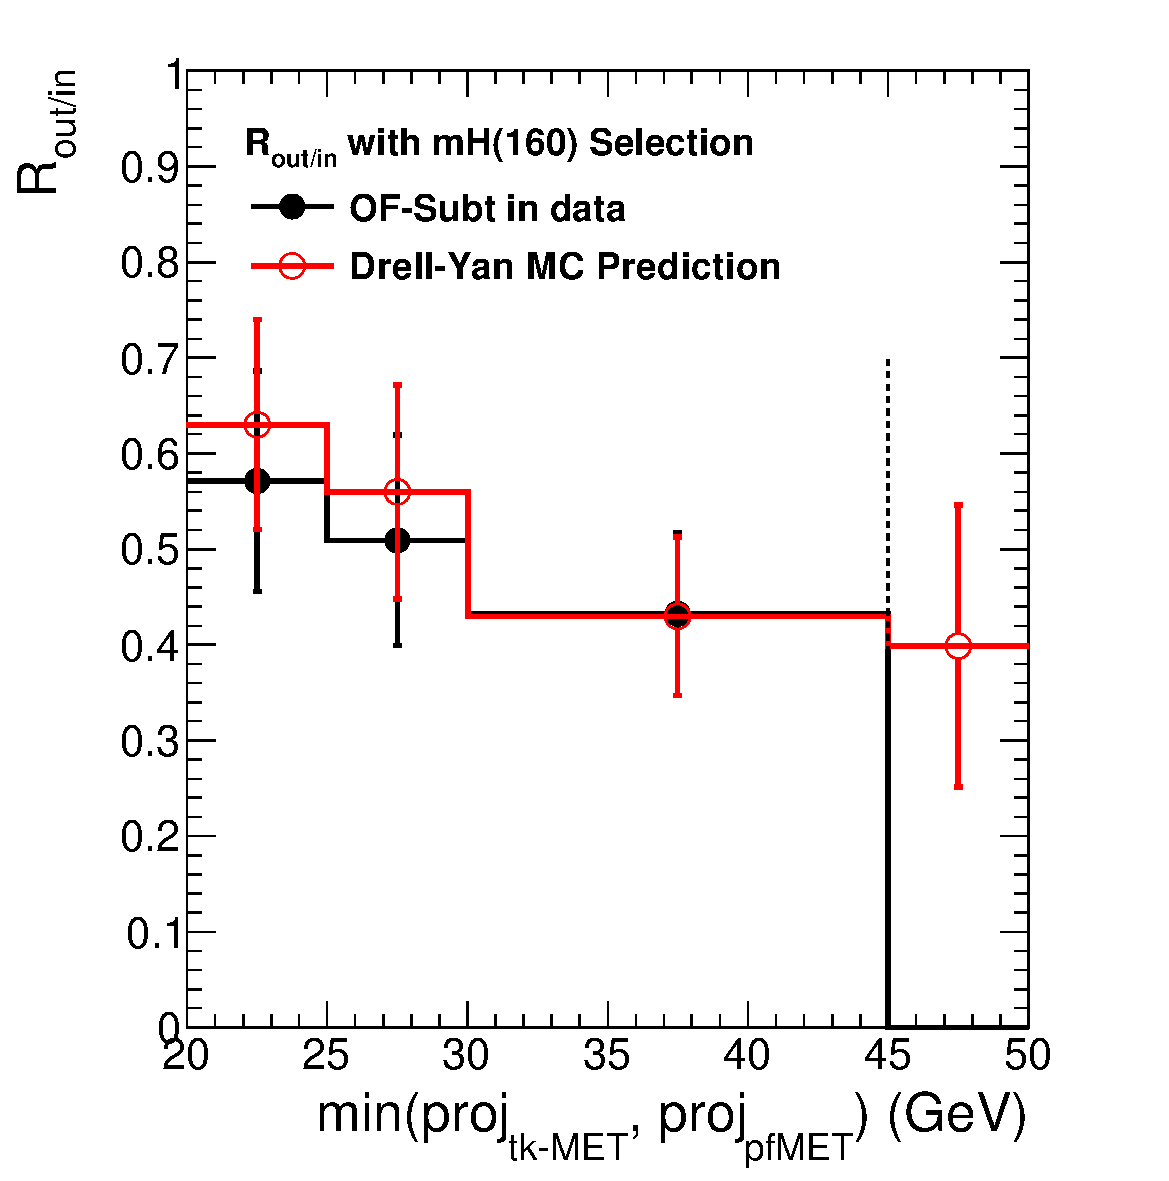
\includegraphics[width=.29\textwidth]{figures/Routin_1Jet_mH160_1616pb_dy.pdf} &
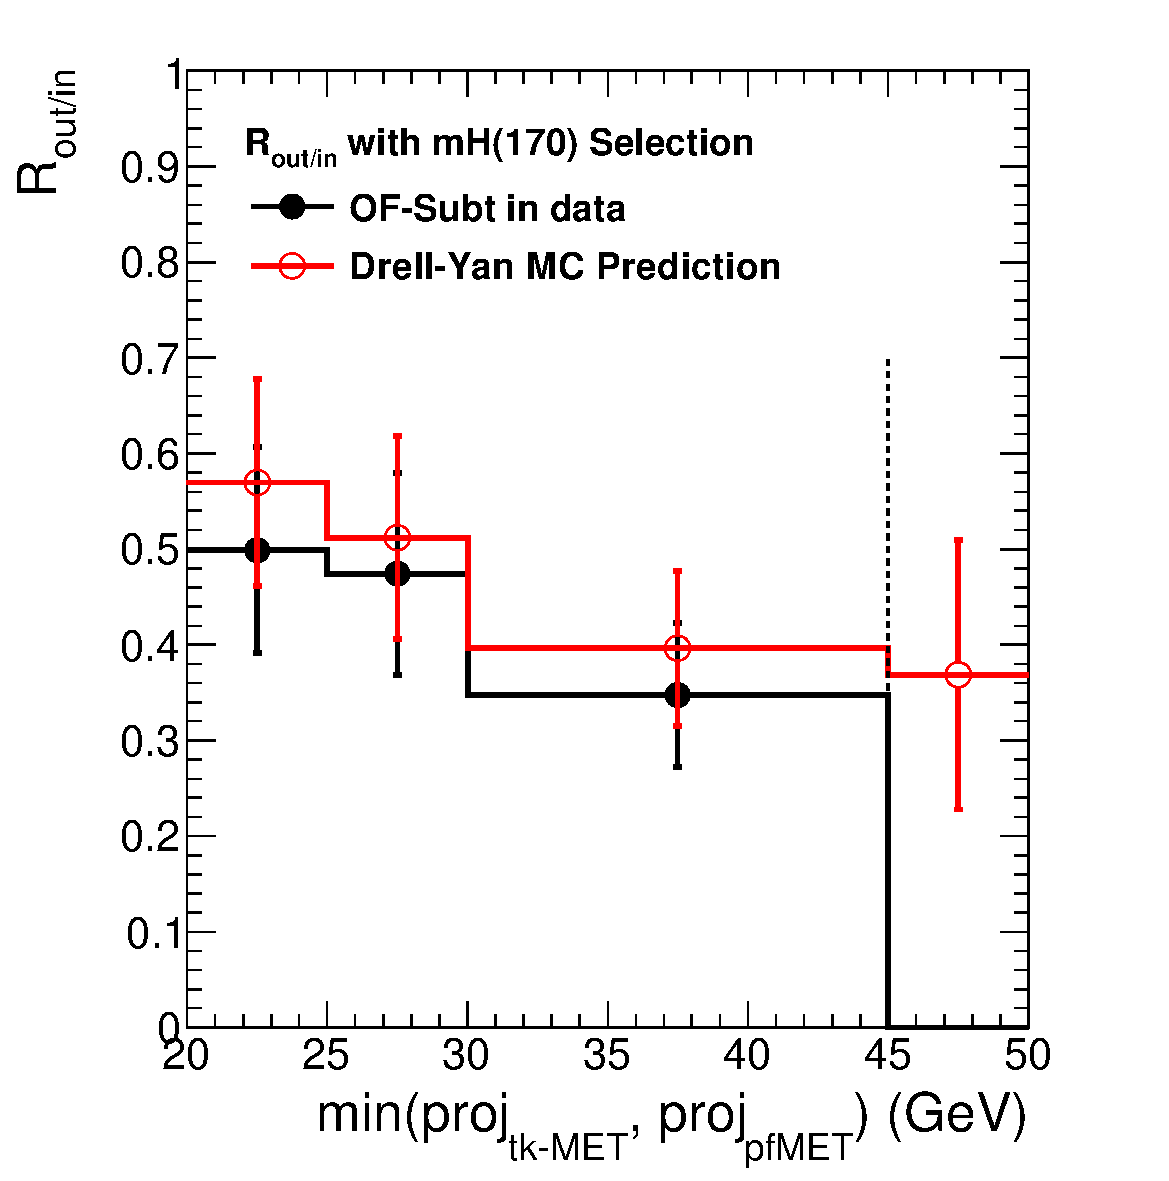
\includegraphics[width=.29\textwidth]{figures/Routin_1Jet_mH170_1616pb_dy.pdf} &
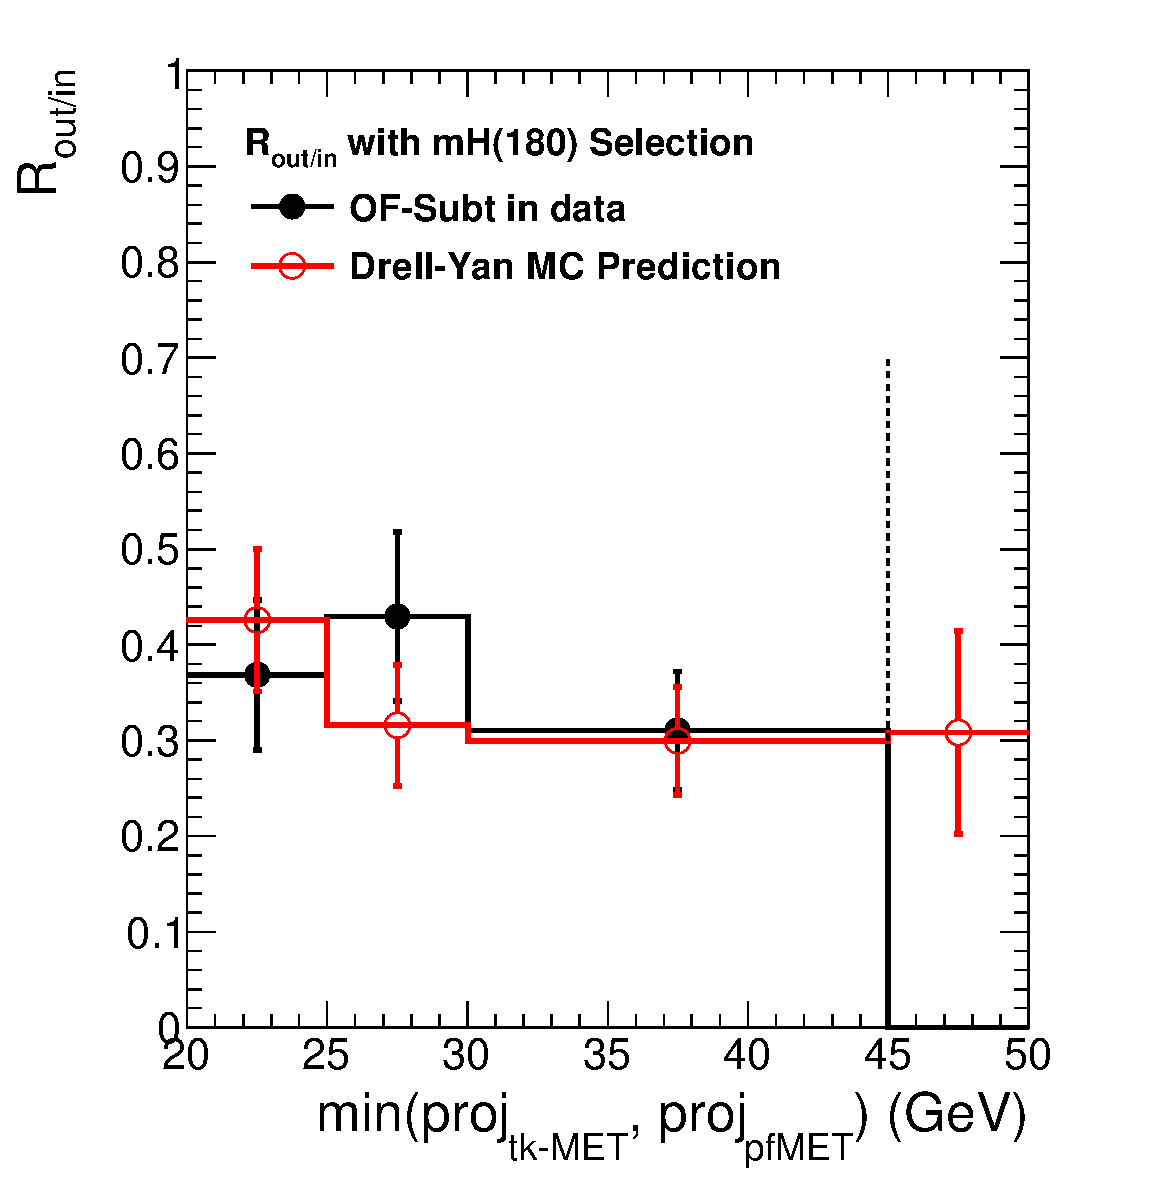
\includegraphics[width=.29\textwidth]{figures/Routin_1Jet_mH180_1616pb_dy.pdf} \\
\end{array}$
\caption{ The \routin\, (ee and $\mu\mu$ combined) as a function of MET measured from data (black solid dots) 
and MC (red open circles) for the Drell-Yan processes in the 1-Jet bin at the 
Higgs selection level in the cut-based analysis. 
The measurements in data are performed using the opposite flavor subtraction method. 
The difference in the \routin measurements in different higg selections are due to the 
different kinematic cuts applied. 
}
\label{fig:routin_1jet}
\end{center}
\end{figure}
